\chapter{An improved framework for downscaling cloud properties from
large-scale models}\label{sec:subgrid2}

The previous chapter identified errors in simulated satellite cloud
diagnostics that arise from using unrealistic cloud overlap assumptions
and horizontally homogeneous condensate. In this chapter, an improved
subcolumn generator is presented, building on the work of previous
investigators, to reduce those errors and enable more consistent and
robust comparisons of modeled and satellite-retrieved cloud statistics.

The improved subcolumn generator described here uses a scheme developed
by \citet{raisanen_et_al_2004} to generate subcolumn cloud condensate
that both follows a more realistic and flexible cloud overlap assumption
and allows for generating subcolumn condensate with horizontal
variability. This scheme has been extended here to apply to
precipitation as well. Using the same framework as in Chapter 3, the new
subcolumn generator presented here is shown to substantially reduced the
identified errors that arise in using SCOPS and PREC\_SCOPS to generate
stochastic subcolumns of cloud and precipitation condensate.

\section{Generating stochastic subcolumns of cloud and precipitation
condensate}\label{sec:subgrid2Generator}

\citet{raisanen_et_al_2004} (hereafter R04) introduce a stochastic
subcolumn cloud generator that can handle both horizontally variable
cloud condensate and generalized cloud overlap. In the R04 scheme,
subcolumn cloud occurrence is first determined by assuming that cloud
overlap between adjacent layers is a linear combination of maximum and
random overlap, such that the combined cloud fraction between two layers
\(k_1\) and \(k_2\) is \begin{equation}\begin{gathered}
    \overline{c}_{k_1, k_2}^\textrm{gen} 
        = \alpha_{k_1, k_2} \overline{c}_{k_1,k_2}^\textrm{max} 
        + (1 - \alpha_{k_1, k_2}) \overline{c}_{k_1, k_2}^\textrm{ran}
\end{gathered}\label{eq:generalized_overlap_equation}\end{equation}
where \(\overline{c}_{k_1, k_2}^\textrm{gen}\) is the combined
(vertically projected) cloud area (fraction) that would result from
generalized overlap, \(\overline{c}_{k_1,k_2}^\textrm{max}\) is the
cloud area that would result if the layers were maximally overlapped,
\(\overline{c}_{k_1, k_2}^\textrm{ran}\) is the cloud fraction that
would result if the layers were randomly overlapped, and
\(\alpha_{k_1, k_2}\) is the ``overlap parameter'' that specifies the
weighting between maximum and random overlap. The theoretical combined
cloud fractions \(\overline{c}^\textrm{max}_{k_1, k_2}\) and
\(\overline{c}^\textrm{ran}_{k_1, k_2}\) are defined as
\[\begin{gathered} 
    \overline{c}^\textrm{max}_{k_1, k_2} 
        = \max(\overline{c}_{k_1},\overline{ c}_{k_2}) \\         
            \overline{c}^\textrm{ran}_{k_1, k_2} 
        = \overline{c}_{k_1} + \overline{c}_{k_2} - \overline{c}_{k_1}         
            \overline{c}_{k_2}
\end{gathered}\] where \(\overline{c}_{k_1}\) and \(\overline{c}_{k_2}\)
are the partial cloud fractions of layers \(k_1\) and \(k_2\),
respectively (i.e., the fraction of the gridbox at levels \(k_1\) and
\(k_2\) that are cloudy).

In general, Equation~\ref{eq:generalized_overlap_equation} is assumed to
apply to any two pairs of layers, but for the practical implementation
of the subcolumn generator R04 consider only adjacent layer pairs. Given
\(\alpha_{k, k-1}\) and the gridbox-mean cloud fraction
\(\overline{c}_{k}\) at each layer \(k\), R04 describe a straightforward
algorithm to stochastically generate a binary subcolumn clear/cloudy
flag with \(n_\textrm{col}\) subcolumns that obeys the above overlap
relationship by stepping down from the top of the atmospheric column and
considering only adjacent layer pairs. First, for each subcolumn \(i\)
and at each level \(k\), three random numbers on the interval \([0, 1)\)
are drawn, denoted \(R1_{i, k}\), \(R2_{i, k}\), and \(R3_{i, k}\). A
variable \(x_{i, k}\) is then generated as follows. At level \(k = 1\)
(TOA), \(x_{i, 1}\) is set to \(x_{i, 1} = R1_{i, 1}\). Levels \(k\) and
columns \(i\) are then iterated over from
\(k = 2, \ldots, n_\textrm{lev}\) and \(i = 1, \ldots, n_\textrm{col}\),
and \(x_{i, k}\) is determined by \[\begin{gathered} 
    x_{i, k} = \begin{cases} 
        x_{i, k-1}, ~ & R2_{i, k} \le \alpha_{k, k-1} \\ 
        R3_{i, k}, ~ & R2_{i, k} > \alpha_{k, k-1}
    \end{cases}
\end{gathered}\] From this, the subcolumn cloudy/clear flag \(c_{i,k}\)
is determined from the value of \(x_{i, k}\) and the partial cloud
fraction \(\overline{c}_{k}\) at level \(k\) by \[\begin{gathered} 
    c_{i, k} = \begin{cases} 
        1, ~ & x_{i, k} > 1 - \overline{c}_{k}, \\ 
        0, ~ & x_{i, k} \le 1 - \overline{c}_{k} 
    \end{cases}
\end{gathered}\]

Once the cloud occurrence subcolumns are created, cloud condensate is
assigned to the cloudy elements by drawing from an assumed probability
distribution for condensate amount. Condensate values are drawn such
that the subcolumn condensate obeys a specified rank correlation
\(\rho_{k, k-1}\) for condensate amount between adjacent layers, where
\(\rho_{k, k-1}\) is the Pearson Product-Moment Correlation coefficient
of the ranks \(r_{k}\) and \(r_{k-1}\) of condensate at levels \(k\) and
\(k-1\), defined by \begin{equation}\begin{gathered} 
    \rho_{k, k-1} = \frac{
        \textrm{cov}(r_{k}, r_{k-1})
    }{
        \sigma_{r_{k}} \sigma_{r_{k-1}} 
    } = \frac{
        \sum_{i=1}^{n_\textrm{col}} (r_{i, k} - \overline{r_{k}})(r_{i, k-1} - \overline{r_{k-1}}) 
    }{
        \sqrt{\sum_{i=1}^{n_\textrm{col}} (r_{i, k} - \overline{r_{k}})^2} \sqrt{\sum_{i=1}^{n_\textrm{col}} (r_{i, k-1} - \overline{r_{k-1}})^2} 
    } \end{gathered}\label{eq:rankcorr_equation}\end{equation} where the
overbars denote horizontal averages over all \(n_\textrm{col}\)
subcolumns. Condensate values are drawn to satisfy a specified
\(\rho_{k, k-1}\) by first generating a variable \(y_{i, k}\) at each
subcolumn \(i\) and level \(k\) analogous to the variable \(x_{i, k}\)
used to determine the binary occurrence flag. Again, three sets of
random numbers \(R4_{i, k}\), \(R5_{i, k}\), and \(R6_{i, k}\) on the
interval \([0, 1)\) are drawn at each subcolumn \(i\) and level \(k\).
The top (\(k = 1\)) layer is set to \(y_{i, 1} = R4_{i, 1}\). For each
subsequent level \(k = 2, \ldots, n_\textrm{lev}\), \[\begin{gathered} 
    y_{i, k} = \begin{cases} 
        y_{i, k-1}, ~ & R5_{i, k} \le \rho_{k-1, k} \\ 
        R6_{i, k},  ~ & R5_{i, k} > \rho_{k-1, k} 
    \end{cases}
\end{gathered}\]

With this, and an assumed probability distribution for condensate amount
with probability density function \(p_k(q)\) at level \(k\), where \(q\)
is the condensate amount (specified as a mass mixing ratio), the
condensate amount \(q_{i, k}\) at each level is determined by finding
\(q_{i, k}\) such that \[\begin{gathered} 
    y_{i, k} = \int_0^{q_{i, k}} p_{k}(q') ~dq'
\end{gathered}\] That is, \(q_{i, k}\) is the mixing ratio at which the
cumulative density function (CDF) of condensate mixing ratios is equal
to \(y_{i, k}\).

The problem of generating stochastic subcolumns of cloud condensate with
generalized occurrence overlap and heterogeneous condensate
distributions then reduces to specifying the parameters
\(\alpha_{k, k-1}\) and \(\rho_{k, k-1}\) for each pair of adjacent
layers within a gridbox, and specifying an appropriate probability
distribution from which to sample condensate amount.

Studies (based largely on cloud radar) have shown that the cloud
occurrence overlap can be fit to an inverse exponential function of the
separation between layers, such that \begin{equation}\begin{gathered} 
    \alpha_{k_1, k_2} = \exp\left(-\frac{z_{k_1} - z_{k_2}}{z_0}\right) 
\end{gathered}\label{eq:alpha_exponential}\end{equation} where
\(z_{k_1}\) and \(z_{k_2}\) are the heights of layers \(k_1\) and
\(k_2\), and \(z_0\) is the ``decorrelation length'' for cloud overlap
that specifies how quickly the vertical correlation in cloud occurrence
decays from maximal to random
\citep{hogan_and_illingworth_2000, mace_and_benson-troth_2002, raisanen_et_al_2004, pincus_et_al_2005, barker_2008, tompkins_and_digiuseppe_2015}.
\citet{raisanen_et_al_2004} and \citet{pincus_et_al_2005} further
suggest that the same exponential relationship can describe the rank
correlation of condensate, but in general using a separate decorrelation
length. These studies have suggested decorrelation lengths for cloud
occurrence overlap between 1.5 and 2.5 km, and somewhat smaller
decorrelation lengths for condensate rank correlation (decorrelations
lengths for rank correlation approximately half those for occurrence
overlap). Overlap and decorrelation lengths will be parameterized in the
following section for use with the SP-CAM output used in this study.

The R04 subcolumn generator as summarized above was designed
specifically for generating stochastic subcolumns of cloud condensate.
However, as shown in the previous chapter, the treatment of subcolumn
precipitation is critical to obtaining reasonable simulations of radar
reflectivity factor from large scale model output. The R04 generator is
extended here to also generate stochastic subcolumns of precipitation
condensate with horizontally heterogeneous condensate amount in order to
also improve the treatment of unresolved precipitation for use with the
simulators.

As an initial approach to extending this subcolumn scheme to handle
precipitation, the subcolumn cloud occurrence \(\tilde{c}_{i, k}\) is
first generated using the subcolumn generator described above. The
subcolumn precipitation occurrence \(\tilde{p}_{i, k}\) is then
generated using the PREC\_SCOPS routine from COSP, with the
precipitation adjustment described in the previous chapter to constrain
the number of precipitating subcolumn elements by the precipitation
fraction from the model. The subcolumn precipitation condensate amount
is then prescribed in a similar manner to the subcolumn cloud condensate
amount but with a separate rank correlation for precipitation, and in
general a separate assumed probability distribution. Other approaches
could certainly be designed to extend this to precipitation, but as
demonstrated in the following sections this simple approach performs
quite well (when the correct cloud occurrence overlap and variability
are used).

This describes a complete subcolumn generator that can produce
subcolumns with generalized cloud occurrence overlap, prescribed
precipitation occurrence fraction, and horizontally heterogeneous cloud
and precipiation condensate, given the occurrence overlap decorrelation
length for cloud, the decorrelation lengths for condensate amount rank
correlation, and assumed probability distributions for cloud and
precipitation condensate amounts. In order to use this generator in a
large-scale, however, these quantities must be parameterized, and
Section~\ref{sec:subgrid2Overlap} and
Section~\ref{sec:subgrid2Variability} describe parameterizing these
quantities for use in the sensitivity study to follow. Because the goal
of this study is to evaluate the sensitivity of the simulated satellite
diagnostics to this new treatment of unresolved cloud and precipitation
structure and variability, these quantities will be parameterized using
a month of output from the SP-CAM. This approach is ideal for this study
because it allows for direct comparison with diagnostics calculated from
the unmodified SP-CAM model output in a similar manner as in Chapter 3,
thus allowing quantification of the sensitivities to these parameters.
However, it is important to recognize that the SP-CAM fields from which
the parameterizations are developed here are model fields, not
observations. As such, the parameterization developed here is subject to
limitations of the model used, and may not be entirely consistent with
observations of clouds in the physical atmosphere. Nonetheless, the
analysis that follows offers a new perspective on overlap and
variability that has not been fully explored in the literature,
providing a global description of both overlap and variability
statistics from a high resolution model. Previous efforts to quantify
overlap have been limited in duration \citep{raisanen_et_al_2004},
limited to smaller domains using cloud resolving models
\citep{pincus_et_al_2005} or ground-based cloud radar
\citep{hogan_and_illingworth_2000, mace_and_benson-troth_2002}, or used
satellite-based studies that come with their own limitations
\citep{barker_2008, oreopoulos_et_al_2012}.

\section{Parameterizing occurrence overlap and rank correlation from
SP-CAM}\label{sec:subgrid2Overlap}

Occurrence overlap and rank correlation are derived from the same SP-CAM
model output used earlier to evaluate sensitivities in COSP diagnostics
to overlap. With the high-resolution model output provided by the
SP-CAM, the occurrence overlap can be directly calculated for each
gridbox from the subcolumn cloud condensate amount by solving
Equation~\ref{eq:generalized_overlap_equation} for \(\alpha_{k_1, k_2}\)
and assuming that the ``true'' combined cloud fraction between layers
\(k_1\) and \(k_2\) can be described by generalized overlap, so that
\(\overline{c}^\textrm{true}_{k_1, k_2} = \overline{c}^\textrm{gen}_{k_1, k_2}\).
This yields for the overlap parameter \(\alpha\)
\begin{equation}\begin{gathered} 
    \alpha_{k_1, k_2} = \frac{
        \overline{c}^\textrm{true}_{k_1, k_2} 
            - \overline{c}^\textrm{ran}_{k_1, k_2} 
    }{
        \overline{c}^\textrm{max}_{k_1, k_2} 
            - \overline{c}^\textrm{ran}_{k_1, k_2} 
    }
\end{gathered}\label{eq:alphaEquation}\end{equation}

For each gridbox and for each pair of layers \(k_1\) and \(k_2\) then,
\(\alpha_{k_1, k_2}\) can be calculated by first calculating the true
combined cloud fraction between the two layers
\(\overline{c}^\textrm{true}_{k_1, k_2}\) and the theoretical maximally
and randomly-overlapped cloud fractions
\(\overline{c}^\textrm{max}_{k_1, k_2}\) and
\(\overline{c}^\textrm{ran}_{k_1, k_2}\), and then using these in
Equation~\ref{eq:alphaEquation}. Using this, overlap is calculated for
pairs of layers in each model gridbox and at each archived 3-hourly
snapshot of the SP-CAM outputs used in the previous chapter. The overlap
calculation is restricted to layers with partial cloud fractions between
5\% and 95\% cloud area. The dependence on the separation between layers
is determined using 40 uniformly-spaced height bins from 0 to 5 km over
the single month of output. The analysis is limited to separations of 5
km or less because layers separated by more than 5 km are essentially
uncorrelated, and considering only those layers separated by 5 km or
less tends to improve the quality of the fit to
Equation~\ref{eq:alpha_exponential} \citep{pincus_et_al_2005}. The
monthly-averaged overlap as a function of separation is then calculated
by summing the binned overlap and dividing by the number of valid counts
in each bin. This is done for each latitude-longitude gridbox and
separation bin. Rank correlation of total cloud and total precipitation
condensate is similarly calculated at each gridbox and level for each
3-hourly snapshot, and binned using the same separation distance bins
used to bin the overlap.

\begin{figure}[htbp]
\centering
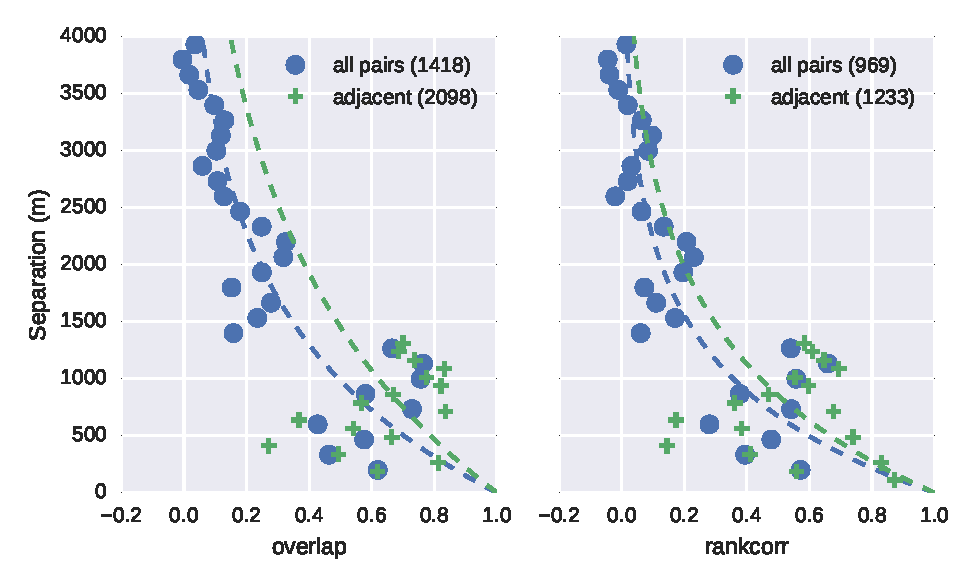
\includegraphics{graphics/subgrid2_overlap_dz.pdf}
\caption{\label{fig:overlap_dz}Global (area-weighted) average cloud
occurrence overlap parameter (left) and condensate rank correlation
(right) as a function of separation distance between layers from a month
of SP-CAM output. Also shown are fits to
Equation~\ref{eq:alpha_exponential}, with values of decorrelation length
scales from these fits shown in the upper right corner of each
panel.}\label{fig:overlapux5fdz}
\end{figure}

Figure~\ref{fig:overlap_dz} shows the globally averaged overlap and
condensate rank correlation for total cloud condensate as a function of
separation distance (the area-weighted average of the overlap and rank
correlation calculated at each latitude-longitude gridbox). Overlap and
rank correlation are fit to Equation~\ref{eq:alpha_exponential} using
non-linear least squares, and the fit is plotted on
Figure~\ref{fig:overlap_dz} as well. Two sets of points and fits are
shown in the figure, corresponding to overlap statistics calculated
using all layer pairs and statistics calculated for only adjacent layer
pairs. The globally averaged overlap and rank correlation statistics
shown in Figure~\ref{fig:overlap_dz} demonstrate the general tendency
for both overlap and rank correlation to decrease as the separation
between layers increases, and especially for distant layers the inverse
exponential dependence on separation distance following
Equation~\ref{eq:alpha_exponential} seems reasonable. There is, however,
generally larger spread in cloud overlap and rank correlation for small
layer separations. This spread in statistics for small separations is
not seen in previous analyses \citep[e.g.,][]{pincus_et_al_2005}, but
those analyses have been primarily limited to much smaller domains, and
presumably consist of a smaller subset of cloud regimes than the global,
month-long simulation considered here. R04 show overlap decorrelation
lengths for a single day of SP-CAM output as a function of latitude and
vertical (pressure) level, and it is evident from that analysis that
overlap statistics vary substantially with both location and height,
with decorrelation lengths varying from less than 0.5 km near the
surface up to 10 km in the upper troposphere (see Figure 3 in R04). Some
amount of spread in Figure~\ref{fig:overlap_dz} can be expected then,
due to grouping all profiles at all levels together. The good agreement
for larger separations is nonetheless expected, however, since
regardless of cloud type distant layers are expected to be uncorrelated
and thus overlap and rank correlation should approach zero (random
overlap and no correlation) as separations become large.

\begin{figure}[htbp]
\centering
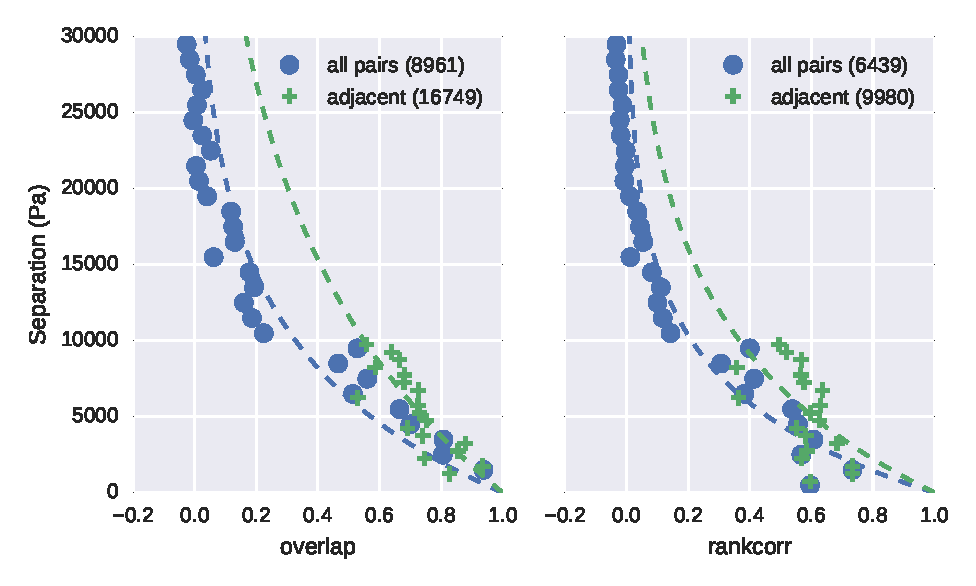
\includegraphics{graphics/subgrid2_overlap_dp.pdf}
\caption{\label{fig:overlap_dp}Global (area-weighted) average cloud
occurrence overlap parameter (left) and condensate rank correlation
(right) as a function of separation in \emph{pressure} between layers
from a month of SP-CAM output. Also shown are fits to
Equation~\ref{eq:alpha_exponential}, with values of decorrelation length
scales from these fits indicated in the legend. Blue markers and curves
correspond to statistics calculated using \emph{all} layer pairs, while
green markers and curves correspond to statistics calculated using only
\emph{adjacent} layer pairs.}\label{fig:overlapux5fdp}
\end{figure}

It is also possible that some of the spread in overlap statistics for
small separations is partly due to the fact that these statistics are
binned using separation in geometric height (altitude), while the model
itself is formulated using a hybrid sigma-pressure grid \citep[the CRM
uses the lowest 24 levels of
CAM;][]{marchand_et_al_2009, collins_et_al_2004}. Parameterizing overlap
in terms of the geometric height separation makes sense for clouds in
the physical atmosphere, but tighter constraints may be realized by
binning overlap statistics on a grid more consistent with the native
model grid. To examine this further, Figure~\ref{fig:overlap_dp} shows
overlap and rank correlation calculated as in
Figure~\ref{fig:overlap_dz} but for total cloud condensate binned by
separation in \emph{pressure} rather than by separation in height
between layer pairs. It is clear that both overlap and rank correlation
in total cloud condensate are fit better when binning by pressure
separation rather than height (less spread in the averages). This is
especially true at small separations and using only adjacent pairs, but
binning by pressure separation seems to improve the quality of the fit
to distant layers as well. However, parameterizing overlap by separation
in pressure rather than by separation in height did not seem to
significantly affect the simulation of COSP diagnostics (not shown), so
overlap statistics will be parameterized by separation in height for
consistency with the existing literature.

There appear to be two distinct groups of points in each panel in both
Figure~\ref{fig:overlap_dz} and Figure~\ref{fig:overlap_dp}, with
different overlap characteristics for separations greater than about 1.3
km (100 hPa) than below. These two groups correspond to distant layer
pairs (layer pairs separated by one or more model layers) and adjacent
layer pairs, respectively. A second set of points is plotted in each
panel of Figure~\ref{fig:overlap_dz} and Figure~\ref{fig:overlap_dp},
showing the overlap and rank correlation calculated using only adjacent
layers (with a separate set of bins than used for all layer pairs in
order to increase the resolution for adjacent pairs). These additional
points show that indeed the two separate groups result from differences
in the overlap characteristics for adjacent versus distant layer pairs.
Fitting Equation~\ref{eq:alpha_exponential} using only adjacent pairs
results in larger decorrelation length scales for both cloud overlap and
rank correlation than when fitting using all pairs.

The differences in overlap and rank correlation statistics for adjacent
and non-adjacent layers mean that parameterizing overlap and rank
correlation is a compromise between reproducing the correct
relationships for adjacent layers versus reproducing the correct
relationships for distant layers. Because the R04 subcolumn generator
only considers relationships between adjacent layers, it might be
possible to achieve better performance by parameterizing overlap and
rank correlation using only adjacent layers as well. However, the
distinction of adjacent and non-adjacent layers is not very meaningful
outside the context of a model, so most efforts to parameterize these
quantities by separation distance have considered all layer pairs.
Furthermore, it might be argued that reproducing the correct overlap
statistics for all layer pairs is more important than reproducing the
correct overlap statistics for only adjacent pairs, if the former has a
larger impact on the resulting vertically projected cloud area. This
probably depends on the amount and nature of multi-layer cloud profiles.
Fundamentally, the ability of the R04 subcolumn generator to faithfully
reproduce both overlap and vertically projected cloud area rests on the
assumption that considering only adjacent layers is sufficient to
reproduce the overall statistics, including the relationships between
distant layers. Thus, parameterizing using all layer pairs, rather than
using only adjacent layer pairs, may help to reduce the impact of this
assumption by explicitly building in the overall statistics.

\begin{figure}[htbp]
\centering
\includegraphics{graphics/subgrid2_overlap_map_dz.pdf}
\caption{\label{fig:overlap_map_dz}Maps of cloud occurrence overlap
(left) and condensate rank correlation (right) decorrelation length
scales for both cloud (top) and precipitation (bottom). Decorrelation
length scales at each point are calculated by fitting time-averaged
overlap and rank correlation as a function of separation in
\emph{height} (meters) to Equation~\ref{eq:alpha_exponential}. White
areas on the map indicate where the fit failed to
converge.}\label{fig:overlapux5fmapux5fdz}
\end{figure}

\begin{figure}[htbp]
\centering
\includegraphics{graphics/subgrid2_overlap_map_dp.pdf}
\caption{\label{fig:overlap_map_dp}Maps of cloud occurrence overlap
(left) and condensate rank correlation (right) decorrelation length
scales for both cloud (top) and precipitation (bottom). Decorrelation
length scales at each point are calculated by fitting time-averaged
overlap and rank correlation as a function of separation in
\emph{pressure} (hPa) to Equation~\ref{eq:alpha_exponential}. White
areas on the map indicate where the fit failed to
converge.}\label{fig:overlapux5fmapux5fdp}
\end{figure}

\begin{figure}[htbp]
\centering
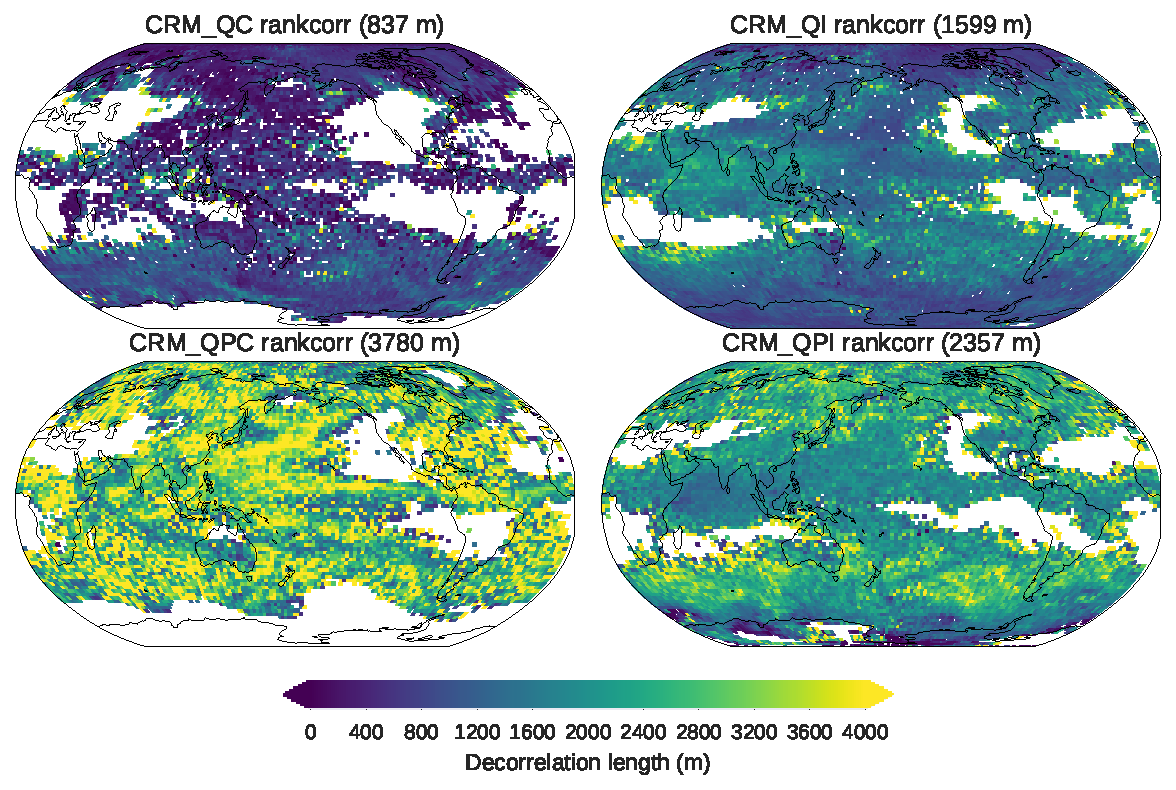
\includegraphics{graphics/subgrid2_rankcorr_maps.pdf}
\caption{\label{fig:rankcorr_maps_dz}Decorrelation lengths for
condensate rank correlation binned by separation in \emph{height} for
cloud liquid (CRM\_QC, upper left), cloud ice (CRM\_QI, upper right),
precipitating liquid (CRM\_QPC, lower left), and precipitating ice
(CRM\_QPI, lower right). White areas on the map indicate where the fit
failed to converge.}\label{fig:rankcorrux5fmapsux5fdz}
\end{figure}

\begin{figure}[htbp]
\centering
\includegraphics{graphics/subgrid2_rankcorr_maps_dp.pdf}
\caption{\label{fig:rankcorr_maps_dp}Decorrelation lengths for
condensate rank correlation binned by separation in \emph{pressure} for
cloud liquid (CRM\_QC, upper left), cloud ice (CRM\_QI, upper right),
precipitating liquid (CRM\_QPC, lower left), and precipitating ice
(CRM\_QPI, lower right). White areas on the map indicate where the fit
failed to converge.}\label{fig:rankcorrux5fmapsux5fdp}
\end{figure}

In order to assess the spatial dependence of cloud occurrence overlap
and condensate rank correlations, time-averaged overlap and rank
correlations are fit to Equation~\ref{eq:alpha_exponential} at each
latitude-longitude gridbox. The decorrelation lengths from the cloud
occurrence overlap fits at each point are shown in
Figure~\ref{fig:overlap_map_dz} and in Figure~\ref{fig:overlap_map_dp}
for overlap binned by separation in altitude and by separation in
pressure, respectively. The subcolumn generator described here allows
for generalized overlap of total cloud occurrence, using only the
overlap parameter between adjacent layers for total cloud. The method of
generating condensate distributions, however, in general allows for
separate rank correlations to be specified for each hydrometeor type
(cloud liquid, cloud ice, precipitating liquid, and precipitating ice).
Thus, rank correlations are calculated separately for each hydrometeor
type from the SP-CAM output, and are also fit to
Equation~\ref{eq:alpha_exponential} at each point. The decorrelation
lengths from these fits are shown in Figure~\ref{fig:rankcorr_maps_dz}
and Figure~\ref{fig:rankcorr_maps_dp} for rank correlations binned by
separation in height and in pressure, respectively.

Decorrelation lengths for both cloud occurrence overlap and condensate
rank correlations vary substantially with geographic location, which
suggests that these overlap statistics are dependent on cloud type.
\citet{pincus_et_al_2005} speculated that overlap and rank correlation
are likely different for convective versus stratiform clouds, and showed
that (for the month long simulation of convection over the ARM SGP site)
convective clouds were more vertically coherent than stratiform clouds.
Based on this argument, it might be expected that occurrence overlap
decorrelation lengths would be systematically larger in more
convectively-active regions. The maps shown in
Figure~\ref{fig:overlap_map_dz} and Figure~\ref{fig:overlap_map_dp} do
not seem entirely consistent with this assumption, however, as
occurrence overlap decorrelation lengths are generally lower throughout
the deep tropics (where deep convective cloud systems are abundant), and
systematically higher throughout the subtropics. These results are,
however, consistent with the results shown by R04 using a single day of
SP-CAM output; Figure 3 in R04 shows zonal-mean decorrelation lengths
for both cloud occurrence and cloud condensate rank correlation as
functions of height (calculated using adjacent layer pairs), and there
are clear local maxima in decorrelation lengths near 30 N and 30 S
throughout the middle troposphere. \citet{oreopoulos_et_al_2012} obtain
a somewhat different result using CloudSat and CALIPSO-retrieved
hydrometeor occurrences from the 2B-GEOPROF-LIDAR product; they find a
clear zonal structure in decorrelation lengths for cloud overlap, with
systematically \emph{higher} decorrelation lengths in the tropics and
\emph{lower} decorrelation lengths in the extratopics (closely
resembling a Gaussian). The \citet{oreopoulos_et_al_2012} result seems
more consistent with a larger frequency of convective cloud systems
throughout the tropics leading to generally larger decorrelation
lengths, but is contradictory to the results shown here and in R04.

There are a number of caveats to note when trying to reconcile these
different results. The \citet{pincus_et_al_2005} study composited
statistics separately for columns deemed convective and for columns
deemed stratiform, isolating the statistics of each. The results shown
here (and in R04), however, contain contributions from a range of cloud
types at each point, and comparing the statistics from different
geographic regions is not sufficient to completely isolate the overlap
statistics specific to certain cloud types. For example, while the
tropics contain more convectively active cloud systems that are expected
to have numerically higher overlap, they also contain a significant
amount of cirrus cloud that may have completely different (numerically
lower) overlap. Cases with exceptionally large or exceptionally small
values of overlap could tend to skew the results, even if the cloud
types associated with those cases are less frequent.

Perhaps more importantly, the sources of cloud condensate information
used for each of these studies are fundamentally different. The results
represented here and those shown in R04 used SP-CAM model output, while
the \citet{oreopoulos_et_al_2012} study used data retrieved from cloud
radar and lidar. This distinction is crucial, because the model results
are able to unambiguously discern between different hydrometeor types,
while results obtained from radar reflectivities cannot reliably
differentiate between clouds and precipitation because precipitation
dominates the signal when present. Thus, the profiles used to derive
cloud occurrence overlap in the \citet{oreopoulos_et_al_2012} study may
very likely contain not only cloud, but also precipitation condensate.
While they note that the presence of precipitation may influence the
determination of condensate rank correlation, it is important to note
here that this would also influence the determination of cloud
occcurrence overlap statistics, because precipitation is expected to be
much more maximally overlapped than cloud. Such a contamination of
``cloud'' profiles by precipitation would explain the increase in
occurrence overlap throughout the tropics, where precipitation
occurrence is generally larger in association with deep convection. So,
these results are likely different because the
\citet{oreopoulos_et_al_2012} results show overlap for the combination
of clouds and precipitation, while the results presented here show
overlap for only cloud. The ability to confidently discriminate between
cloud and precipitation statistics with a high resolution model like
that used here should be viewed as a real strength in using this
technique to derive overlap statistics, because it is straightforward to
quantify statistics separately for different hydrometeor types. While
the results obtained using such model results may be subject to
additional questions regarding the fidelity of the model simulation
itself, they do thus provide a complementary description of the overlap
statistics not possible with available observations.

Regardless of these caveats, the spatially varying patterns in
decorrelation lengths for both cloud occurrence overlap and condensate
rank correlation suggest that assuming spatially invariant decorrelation
lengths will likely lead to spatially varying errors in cloud area. This
is shown to be the case in the following sections. However, the goal of
this study is to evaluate the sensitivity to these assumptions relative
to using the maximum-random overlap assumption with horizontally
homogeneous condensate, rather than to derive a comprehensive
parameterization that can be immediately used by default in COSP. For
simplicity then, spatially invariant decorrelation length scales for
both cloud occurrence overlap and for condensate rank correlation are
taken from the cosine-latitude-weighted global mean values, indicated
above each panel in Figure~\ref{fig:overlap_map_dz} and
Figure~\ref{fig:rankcorr_maps_dz}.

\section{Parameterizing cloud and precipitation condensate
variability}\label{sec:subgrid2Variability}

In order to use the R04 scheme to generate subcolumns of cloud and
precipitation condensate with horizontally variable condensate, both the
assumed distribution of condensate and the variance in subcolumn
condensate must be specified. Because these details are not typically
specified in large-scale models, a simple parameterization is discussed
here.

Various aspects of the statistical distribution of condensate have been
quantified using a variety of data sources, including aircraft
observations \citep{wood_and_field_2000, larson_et_al_2001}, tethered
balloon observations \citep{price_2001}, satellite retrievals using
passive sensors \citep{barker_et_al_1996} and more recently using
CloudSat retrievals \citep{lee_et_al_2010}, and using high resolution
model simulations from cloud resolving models and large eddy simulations
\citep{lewellen_and_yoh_1993, xu_and_randall_1996a, xu_and_randall_1996b}.
The primary motivation for these studies has been to parameterize the
distribution of condensate for use in large-scale models. It is
important that such a parameterization is consistent with clouds in the
physical atmosphere so as to have a parameterization that is as
realistic as possible. Thus, it is often desireable to use high-quality
observations to derive these parameterizations. For this study, however,
it is most important that the parameterization is consistent with clouds
simulated by SP-CAM, rather than with observations of clouds, because
the goal of this study is to test the ability of the subcolumn generator
to reproduce subcolumn statistics from the SP-CAM. Because of this, the
parameterization developed here is based entirely on output from the
SP-CAM. While caution should be exercised in trying to use this
parameterization beyond the sensitivity studies presented here without
further evaluation against observations, the use of SP-CAM output to
derive such parameterizations provides distinct advantages over the
approaches used previously, which will be discussed.

Cloud condensate distributions have been fit with a number of different
statistical distributions. \citet{larson_et_al_2001} fit aircraft
observations of the conserved quantity \(s\) (related to the total
specific humidity and saturation specific humidity and suitable for use
in statistical cloud schemes) to various distributions, including single
and double ``delta'' distributions (no variability), the generalized
(3-parameter) gamma distribution, and various iterations of single and
double gaussian distributions. They find that \(s\) is fit well by the
multi-parameter double gaussian distributions, but also find good
agreement with the generalized gamma distribution. More recently,
\citet{lee_et_al_2010} fit retrievals of cloud liquid water content from
CloudSat to a selection of different distributions, including gamma,
lognormal, exponential, gaussian, Weibull, beta, and uniform. They find
that the CloudSat retrievals most closely follow either a lognormal or
gamma distribution (depending on a number of conditions including
geolocation, altitude, temperature, and the presence of precipitation).
They also note that the data is reasonable well fit by the beta
distribution, and \citet{oreopoulos_et_al_2012} subsequently use the
beta distribution in their parameterization of subgrid-scale
variability.

These studies suggest that the gamma distribution is a reasonable fit to
observed distributions of cloud condensate, and it turns out that cloud
and precipitation condensate distributions simulated by the SP-CAM are
also fit well using the gamma distribution. Figure~\ref{fig:mxratioCDF}
shows the empirical cumulative density function (CDF) for normalized
cloud and precipitation condensate \(q / \overline{q}\) for a single day
of SP-CAM output, accumulated over all columns and levels, along with
fits to the gamma distribution. The normalized condensate amount is used
here because the global distribution of condensate is dominated by the
gridbox-mean condensate. Scaling by the mean highlights the
within-gridbox or subgrid-scale variations, which is the type of
heterogeniety that needs to be parameterized. Qualitatively, the gamma
CDF fits agree reasonably well with the empirical CDFs, suggesting that
the gamma distribution is reasonably consistent with condensate
distributions generated by the SP-CAM and it is shown later in the
chapter that the resulting simulator output using the new subcolumn
generator represents a significant improvement over SCOPS where
variability is ignored.

\begin{figure}[htbp]
\centering
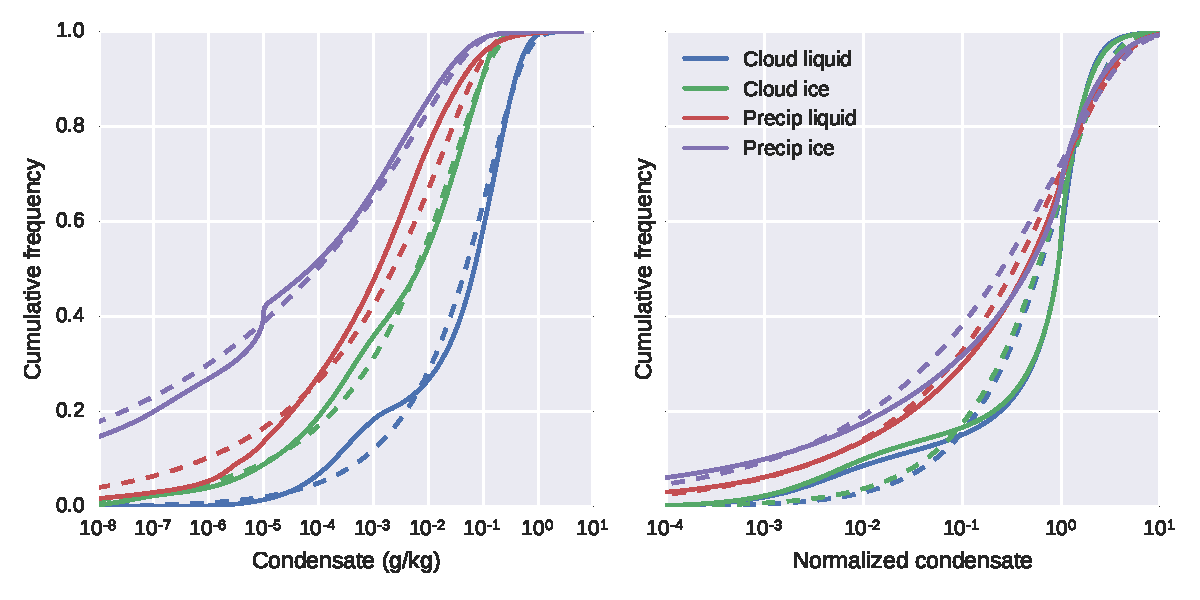
\includegraphics{graphics/subgrid2_mxratio_cdf1.pdf}
\caption{\label{fig:mxratioCDF}Raw (left) and normalized (right) cloud
and precipitation condensate mixing ratio empirical cumulative density
functions (solid curves), with fits to the gamma distribution (dashed
curves) for a single snapshot of SP-CAM output.}\label{fig:mxratioCDF}
\end{figure}

The gamma distribution has probability density \[\begin{gathered} 
    p_{k, \theta}(q) 
        = \frac{1}{\Gamma(k) \theta^k} q^{k - 1} e^{-q/\theta}
\end{gathered}\] where \(q\) is the condensate amount (mixing ratio),
\(k\) and \(\theta\) are the shape and scale parameters of the gamma
distribution, and \(\Gamma\) is the gamma function. The distribution has
mean \(\mu = k\theta\) and variance \(\sigma^2 = k \theta^2\). Using the
method of moments \citep[e.g.,][]{wilks_2011} and equating the
population mean and variance with the sample mean \(\overline{q}\) and
variance \(\sigma_q^2\), this system of two equations is easily solved
to estimate the shape and scale parameters \(k = \mu^2 / \sigma_q^2\)
and \(\theta = \sigma_q^2 / \mu\). Using this formulation, the subgrid
distribution of condensate within each grid-box is completely specified
in terms of the grid-box mean and variance of condensate.

Cloud physics parameterizations in large-scale (global) models diagnose
the gridbox-mean cloud condensate amount, but most do not diagnose (or
even implicitly assume) the gridbox-variance. Again a variety of
observations have been used to study the gridbox-scale variance (or
``heterogeniety''), including aircraft observations, satellite
retrievals, and ground-based retrievals from the CloudNet and ARM sites.
One way of quantifying heterogeniety is by calculating the coefficient
of variation \(\sigma_x / \overline{x}\), where \(\sigma_x\) and
\(\overline{x}\) are the standard deviation and the mean of a quantity
\(x\) (such as cloud condensate amount). The coefficient of variation,
often referred to as the fractional or relative standard deviation, has
been used by other authors to quantify heterogenienty in cloud
condensate
\citep{hogan_and_illingworth_2003, shonk_et_al_2010, hill_et_al_2012, boutle_et_al_2014}.
\citet{shonk_et_al_2010} conclude that a fixed coefficient of variation
is sufficient to specify the heterogeniety, with a value of
\(0.75 \pm 0.18\). This would imply that the gridbox standard deviation
in cloud condensate can be simply specified by scaling the gridbox mean.
However, \citet{hill_et_al_2012} and \citet{boutle_et_al_2014} suggest
that the coefficient of variation varies with cloud fraction. This
suggests that the scaling between gridbox mean and standard deviation in
cloud condensate might depend on the cloud fraction.
\citet{oreopoulos_et_al_2012}, in developing a simple parameterization
to test the sensitivity of radiative fluxes to heterogeniety in a GCM,
also state an observed dependence on cloud fraction using CloudSat
retrievals, although those results were not shown explicitly in the
manuscript. \citet{hill_et_al_2015} suggest that the coefficient of
variation also has a regional dependence, with more heterogeniety in ice
clouds in regions dominated by convection. \citet{lebsock_et_al_2013}
similarly show a regional dependence, with more heterogeniety in the
tropics than in the extratropics. \citet{ahlgrimm_and_forbes_2016}
futher suggest a regime dependence on the heterogeniety.

While these studies have all been based on observations of clouds in the
physical atmosphere, again for the purpose of this study it is most
important that the parameterization is consistent with clouds simulated
by SP-CAM. Thus, condensate variance will be parameterized based on
output from the SP-CAM in this study. While the results of many of these
studies suggest that cloud condensate heterogeniety in the physical
atmosphere may be better parameterized in terms of more than just the
condensate mean, the results of \citet{shonk_et_al_2010} suggest that a
reasonable first attempt might be to represent the condensate standard
deviation in terms of the gridbox mean alone (note that a constant
coefficient of variation imples a linear dependence of standard
deviation on the mean).

Figure~\ref{fig:subgrid2_mxratio_variance} shows the standard deviation
in cloud liquid (upper left), cloud ice (upper right), precipitating
liquid (lower left) and precipitating ice (lower right) condensate
mixing ratios versus gridbox mean cloud and precipitation condensate,
respectively, again for a single snapshot of SP-CAM output. Rather than
show the scatter plot of the standard deviation versus the mean, the
figure shows a kernel density estimate for the bivariate PDF of mean and
standard deviation (shown by the contours). Because the distribution of
the mean and standard deviation of condensate mixing ratios is strongly
skewed, these are shown on a log-log scale. The figure shows that the
standard deviation of condensate is strongly correlated with the mean,
following an approximately linear relationship in log-log space. This
suggests that the standard deviation \(\sigma\) can be represented in
terms of the mean \(\mu\) for each condensate type by the relationship
\begin{equation}\begin{gathered}
    \sigma = a \mu^b
\end{gathered}\label{eq:sigmaMu}\end{equation} where \(a\) and \(b\) are
constants that need to be parameterized. Note that taking the logarithm
of both sides shows that this leads to a linear relationship in log-log
space: \[\begin{gathered} 
    \log \sigma = \log(a \mu^b) = \log a + b\log \mu
\end{gathered}\] Note also that for \(b = 1\), this relationship reduces
to the definition for the coefficient of variation used in the studies
discussed above, with \(a = \sigma / \mu\).

\begin{figure}[htbp]
\centering
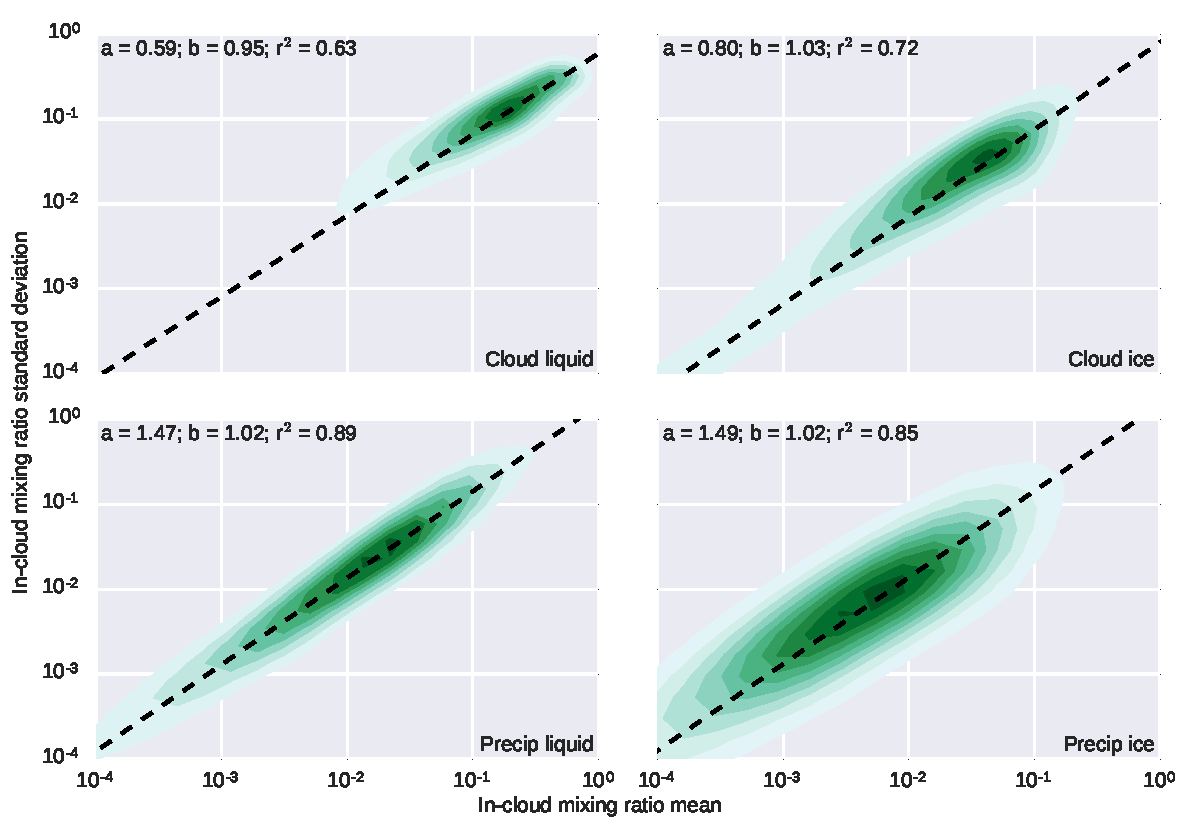
\includegraphics{graphics/subgrid2_mxratio_variance.pdf}
\caption{\label{fig:subgrid2_mxratio_variance}Kernel density estimate
for the bivariate PDF of condensate standard deviation and mean for
cloud liquid, cloud ice, precipitating liquid, and precipitating ice
(contours) for a single global snapshot of SP-CAM CRM output. Shown in
the upper left corner of each panel are the parameters for the fit to
Equation~\ref{eq:sigmaMu}, along with the coefficient of determination
(\(r^2\)) of the fit.}\label{fig:subgrid2ux5fmxratioux5fvariance}
\end{figure}

Standard deviation is fit to \(\sigma = a \mu^b\) by performing a linear
regression of \(\log\sigma\) versus \(\log \mu\) to estimate the slope
and intercept \(a^{\prime}\) and \(b^{\prime}\) in
\(\log \sigma = a^{\prime} \log \mu + b^{\prime}\), and then determining
\(a\) and \(b\) such that \(\sigma = a \mu^b\) by taking
\(a = 10^{b^{\prime}}\) and \(b = a^{\prime}\). That is, the fit is
performed in log-log space, and the fit parameters are then transformed
back. The fit parameters \(a\) and \(b\), as well as the coefficient of
determination \(r^2\) (from the linear regression in log-log space) are
indicated in each panel of Figure~\ref{fig:subgrid2_mxratio_variance}
for the example SP-CAM snapshot. This fit is repeated for each 3-hourly
snapshot of SP-CAM output in the month of July 2000 (248 total
snapshots), and the fit parameters for each snapshot are shown in
Figure~\ref{fig:subgrid2_mxratio_variance_fits}. The fit parameters are
then averaged over all of the snapshots to provide a single
parameterization of the scale and power parameters \(a\) and \(b\) for
use in the sensitivity tests in this chapter, and are shown in
Table~\ref{tbl:subgrid2_mxratio_variance_fits_table}.

\begin{figure}[htbp]
\centering
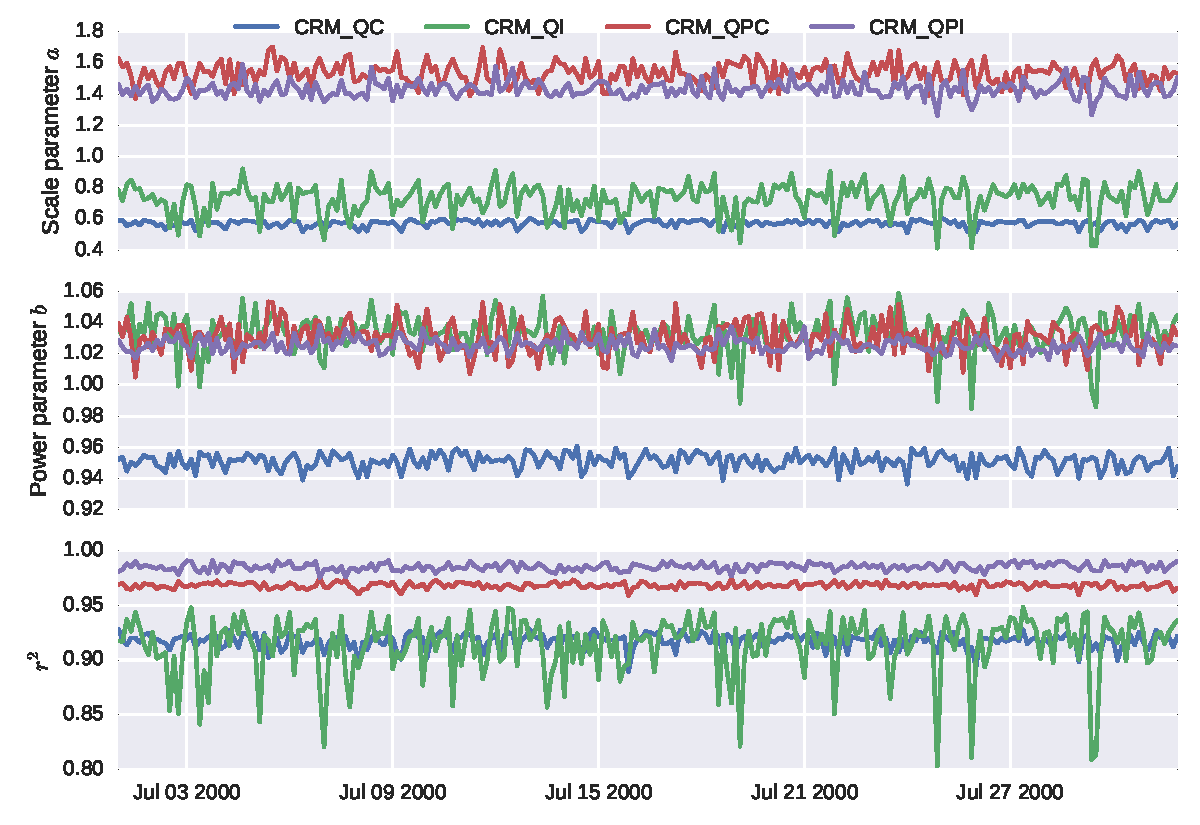
\includegraphics{graphics/subgrid2_mxratio_variance_fits.pdf}
\caption{\label{fig:subgrid2_mxratio_variance_fits}Fits to
Equation~\ref{eq:sigmaMu} for each of the 248 SP-CAM snapshots in July
2000.}\label{fig:subgrid2ux5fmxratioux5fvarianceux5ffits}
\end{figure}

The averages of the power parameters (\(b\)) are all around a value of
\(b = 1\). This suggests that variance might be nearly as well
represented by simply parameterizing the coefficient of variation
directly rather than including the additional parameter \(b\), but
including \(b\) does improve the quality of the fit somewhat.
Regardless, since the average power parameters are near unity, the
values of the scale parameters can be assumed to approximate the
coefficient of variation, since \(\sigma = a \mu^b\) reduces to
\(a = \sigma / \mu\) for \(b = 1\). The averages of the scale parameters
\(a\) for cloud liquid and cloud ice are \(0.57\) and \(0.73\),
respectively. These values are within the range of values found by
\citet{shonk_et_al_2010} for the coefficient of variability using a
variety of observations, suggesting that the variability in the SP-CAM
(and the parameterization developed here) is at least somewhat
consistent with variability in the physical atmosphere.

The fits to Equation~\ref{eq:sigmaMu} shown in
Table~\ref{tbl:subgrid2_mxratio_variance_fits_table} provide a simple
parameterization for condensate standard deviation, so that given the
gridbox mean values at each level, condensate standard deviation can be
represented using the functional relationship Equation~\ref{eq:sigmaMu}.
Assuming constant values for the fit parameters is analogous to assuming
a constant coefficient of variability for condensate, as suggested by
\citet{shonk_et_al_2010}. While more recent studies have shown that
condensate variability likely depends on at least cloud fraction and
cloud regime as well, assuming constant values for these fits provides a
simple parameterization and is a natural starting point for testing the
sensitivity of the COSP diagnostics to horizontal variability. The
dependence of these fit parameters on cloud fraction was briefly
explored, and preliminary results suggest that especially the scale
parameter \(a\) does vary with cloud fraction. However, no clear
functional relationship emerged for use in the parameterization, so it
is left for future work to explore this dependence using model output to
compliment the observational studies.

\begin{longtable}[]{@{}lccc@{}}
\caption{\label{tbl:subgrid2_mxratio_variance_fits_table}Averages of the
fit parameters shown in Figure~\ref{fig:subgrid2_mxratio_variance_fits}
over all 248 SP-CAM snapshots. }\tabularnewline
\toprule
Hydrometeor & Average \(a\) & Average \(b\) & Average
\(r^2\)\tabularnewline
\midrule
\endfirsthead
\toprule
Hydrometeor & Average \(a\) & Average \(b\) & Average
\(r^2\)\tabularnewline
\midrule
\endhead
Cloud liquid & 0.57 & 0.95 & 0.92\tabularnewline
Cloud ice & 0.73 & 1.03 & 0.91\tabularnewline
Precip liquid & 1.54 & 1.03 & 0.97\tabularnewline
Precip ice & 1.43 & 1.03 & 0.99\tabularnewline
\bottomrule
\end{longtable}

\section{Quantifying improvements in COSP-simulated
diagnostics}\label{sec:subgrid2Results}

With the improved subcolumn generator and parameterizations described in
the preceding sections, the sensitivity of the COSP diagnostics to the
improvements can be quantified using the same framework presented in the
previous chapter for quantifying the sensitivities to the maximum-random
overlap and homogeneous condensate assumptions. Again, a set of modified
cloud and precipitation condensate fields are created from a month-long
SP-CAM simulation, COSP is run on each set of modified fields, and the
COSP outputs are compared with one another to quantify the sensitivity
to different aspects of the improved subcolumn generator. These cases
are described below, and illustrated for an example gridbox in
Figure~\ref{fig:mxratioExample2}. The cases are also summarized in
Table~\ref{tbl:subgridCases}.

\begin{figure}[htbp]
\centering
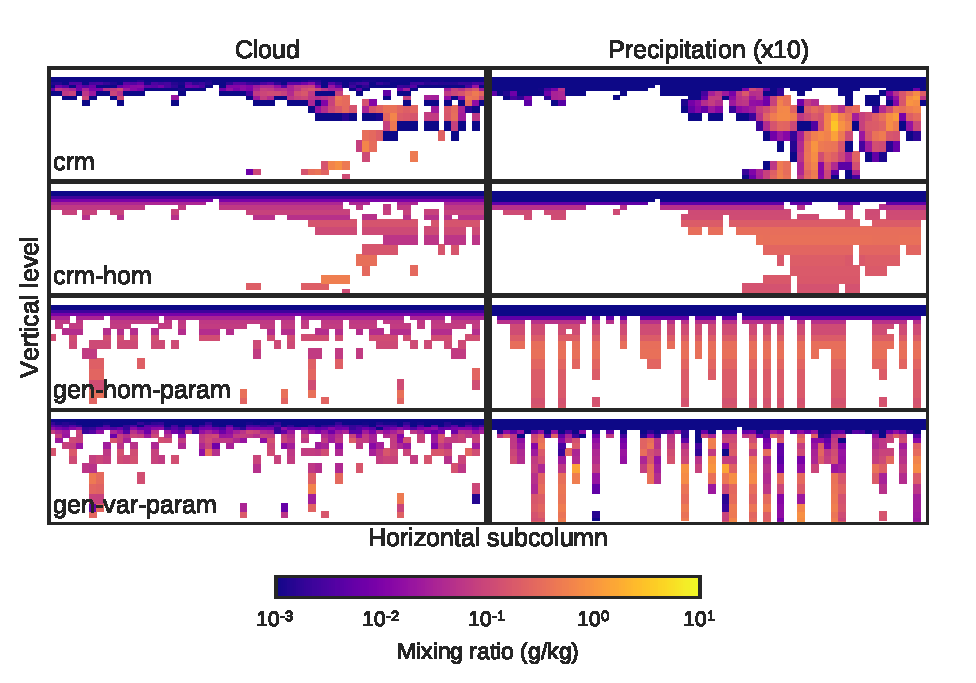
\includegraphics{graphics/subgrid2_mxratio_example.pdf}
\caption{\label{fig:mxratioExample2}Cases with improved subcolumn
generator following R04.}\label{fig:mxratioExample2}
\end{figure}

The first two cases are identical to those used Chapter 3. The first is
created by using the unmodified CRM fields from the SP-CAM, and is
referred to as the ``CRM'' or ``original'' case. The COSP outputs from
this case serve as the baseline against which the performance of the
modified cases is assessed. This case is illustrated for the example
gridbox in the top panels of Figure~\ref{fig:mxratioExample2}. The
second case is created by homogenizing the cloud and precipitation
condensate amounts: condensate amount for each hydrometeor type is
replace with the (horizontal) gridbox-means (by level) everywhere that
condensate type exists in the original CRM fields. Again, this case is
referred to as the ``CRM-HOM'' (exact overlap from the CRM but
homogenized condensate) or the ``homogenized'' case. This case is
illustrated for the example gridbox in the second panel of
Figure~\ref{fig:mxratioExample2}.

\begin{longtable}[]{@{}lll@{}}
\caption{\label{tbl:subgridCases}Treatment of overlap and variance for
each of the modified cases. See text for description of each case.
}\tabularnewline
\toprule
Case & Overlap & Variance\tabularnewline
\midrule
\endfirsthead
\toprule
Case & Overlap & Variance\tabularnewline
\midrule
\endhead
CRM & Exact & Exact\tabularnewline
CRM-HOM & Exact & Homogeneous\tabularnewline
GEN-VAR-PARAM & Parameterized & Parameterized\tabularnewline
GEN-HOM-PARAM & Parameterized & Homogeneous\tabularnewline
GEN-VAR-CALC & Calculated & Calculated\tabularnewline
GEN-HOM-CALC & Calculated & Homogeneous\tabularnewline
\bottomrule
\end{longtable}

The remaining cases are created in a similar manner as in Chapter 3:
gridbox-mean profiles of cloud fraction, precipitation fraction, and
condensate amount (mixing ratio) are calculated from the original CRM
fields and then fed into various renditions of the improved subcolumn
generator described here to regenerate subcolumn condensate fields.
These cases are broadly referred to as the ``regenerated'' cases because
they are attempts to regenerate the full distribution of condensate in
the original CRM fields from the gridbox-means, but different cases are
generated with varying degress of parameterization of overlap, rank
correlation, and heterogeniety in order to test the sensitivity to these
parameterizations.

The first of these regenerated cases uses the full subcolumn generator
described here, with the parameterization of overlap \(\alpha\), rank
correlation \(\rho\), and gridbox standard deviation in condensate
\(\sigma_q\) discussed. This case is referred to as the
``GEN-VAR-PARAM'' case, because it uses the full generator with
generalized overlap and horizontally variable condensate. This case is
illustrated for the example gridbox in the bottom panel of
Figure~\ref{fig:mxratioExample2}. Differences in the outputs between
this case and the original CRM case quantify the total error inherent in
using the full subcolumn generator with parameterized overlap, rank
correlation, and variability.

In order to separate the errors due to the treatment of overlap from
those that arise due to the treatment of variability, another
regenerated case is created that uses the improved subcolumn generator
to account for the occurrence overlap, but which uses horizontally
homogeneous condensate instead of using the parameterization for
horizontal variability. This case is referred to as the
``GEN-HOM-PARAM'' case because it uses generalized overlap but with
horizontally homogeneous condensate amounts. This case is illustrated in
the third panel of Figure~\ref{fig:mxratioExample2}. Because this case
differs from the homogenized (CRM-HOM) case only in the treatment of
occurrence overlap, differences between these two cases represent errors
arising solely due to the parameterization of overlap.

The parameterization of horizontal variability is shown below to be
somewhat less than ideal, so it is not expected that the regenerated
(GEN-VAR-PARAM) case will perfectly reproduce the characteristics of the
original CRM case. Rather, this case represents the performance that can
be expected from the R04 generator with a very simple parameterization
of overlap, rank correlation, and heterogeniety. In order to test the
theoretical limit of performance that can be expected using the R04
generator with ideal parameterization of these quantities, another case
is created that uses the full generator, but with overlap, rank
correlation, and condensate variance \emph{calculated} at each gridbox
and time step directly from the original CRM fields rather than
parameterized. This case is referred to as the ``GEN-VAR-CALC'' case.
Because this case uses the R04 scheme but with overlap, rank
correlation, and variance calculated directly rather than parameterized,
this cases represents the upper limit of the performance that can be
expected from this subcolumn scheme, if these parameters could be
perfectly prescribed. The distribution of subcolumn cloud and
precipitation condensate looks qualitatively similar between the
GEN-VAR-CALC and GEN-VAR-PARAM cases, so the GEN-VAR-CALC case is
omitted from Figure~\ref{fig:mxratioExample2}. In order to separate the
effect of the treatment of occurrence overlap from that of variability,
another case is created using the subcolumn generator to account for
occurrence overlap, with overlap \(\alpha\) calculated directly from the
original CRM fields but with homogeneous condensate. This case, referred
to as the ``GEN-HOM-CALC'' case, is identical to the GEN-HOM-PARAM case
but with calculated rather than parameterized overlap. Again, because
this case is similar to the GEN-HOM-PARAM case already shown, it is
omitted from Figure~\ref{fig:mxratioExample2}. Because this case differs
from the homogenized (CRM-HOM) case only in the treatment of overlap,
differences between these two cases represent errors that can be
expected due to overlap alone, even with perfect parameterization of
overlap.

\begin{figure}[htbp]
\centering
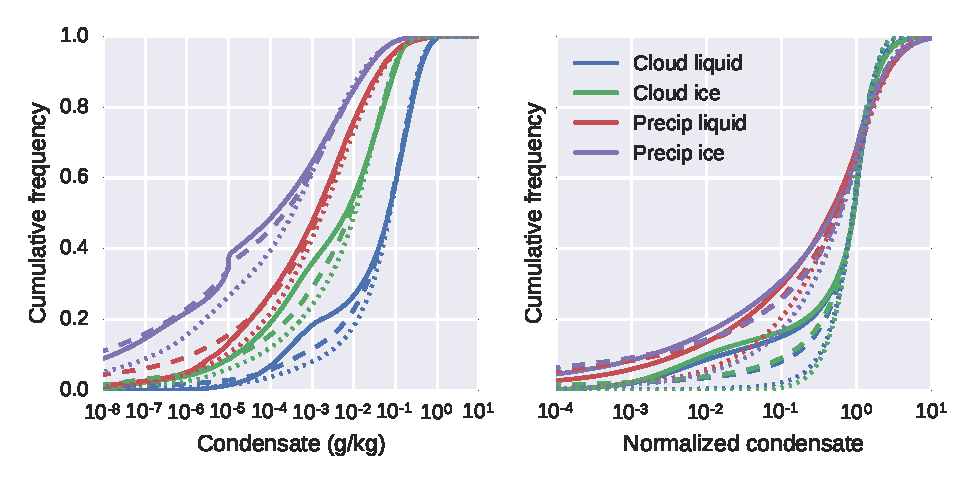
\includegraphics{graphics/subgrid2_mxratio_cdf2.pdf}
\caption{\label{fig:mxratioCDF2}Raw (left) and normalized (right)
condensate empirical density functions from the CRM (solid curves),
GEN-VAR-PARAM (dotted curves), and GEN-VAR-CALC (dashed curves) cases as
described in the text for a single snapshot of SP-CAM
output.}\label{fig:mxratioCDF2}
\end{figure}

Figure~\ref{fig:mxratioCDF2} shows the cumulative distributions of
condensate amounts for each hydrometeor type from the regenerated
GEN-VAR-PARAM (dotted curves) and GEN-VAR-CALC (dashed curves) cases for
a single snapshot of SP-CAM output, compared with the CDFs from the
original CRM fields (solid curves) as shown in
Figure~\ref{fig:mxratioCDF}. The figure shows that the GEN-VAR-CALC case
is able to reasonably reproduce the distribution of both the raw
condensate and of the normalized condensate for each hydrometeor type.
The distributions from the GEN-VAR-PARAM case (using the
parameterization for variance described above) also reproduce the raw
condensate reasonably well, but do not do as well at reproducing the
distribution of normalized condensate for any hydrometeor type. In
general the parameterization tends to underestimate the number of
hydrometeors with very small values relative to the mean, with larger
values of condensate mixing ratios making up the majority of the
distribution. The cause of the relatively poor performance of the
parameterization is not yet known, but it should be noted that this
parameterization is extremely simplified, and better performance may be
had using a more sophisticated treatment (as suggested by the better
agreement using the calculated variance). In particular, building in a
dependence on hydrometeor occurrence fraction and either geolocation or
cloud regime may improve the agreement with the CRM distributions.
Regardless, it is clear that representing variance in terms of the mean
using the (overly simple) parameterization described here will likely
lead to remaining errors in COSP outputs. This is shown to be the case
in the following sections. It should be emphasized again, however, that
the primary goal of this study is to understand the sensitivity of the
COSP outputs to parameterization of overlap and variability.

The sensitivity to both the overlap and the variability treatment can be
quantified by taking appropriate differences between the outputs from
these different cases. The CRM-HOM and GEN-HOM-PARAM (and GEN-HOM-CALC)
cases differ primarily in the treatment of cloud (and precipitation)
overlap, so the difference between the outputs from these cases
quantifies the component of the error due to the generalized overlap
treatment alone. This will be calculated for both the GEN-HOM-CALC case
and for the GEN-HOM-PARAM case, showing both the generalized overlap
errors that can be achieved with ideal overlap and with overlap
specified only by a monthly and spatially invariant (averaged)
decorrelation length. The component of the error due to the treatment of
variability is quantified by calculating the residual between the total
error in using the full subcolumn generator (GEN-VAR-CALC or
GEN-VAR-PARAM minus CRM) and the component of the error due to the
treatment of overlap (GEN-HOM-CALC or GEN-HOM-PARAM minus CRM-HOM). The
total error \(E_\textrm{total}\) and the overlap and variability
components \(E_\textrm{overlap}\) and \(E_\textrm{var}\) are calculated
for a simulated satellite diagnostic quantity \(X\) then as
\[\begin{gathered} 
    E_\textrm{total} = X_\textrm{GEN-VAR} - X_\textrm{CRM} \\ 
    E_\textrm{overlap} = X_\textrm{GEN-HOM} - X_\textrm{CRM-HOM} \\ 
    E_\textrm{var} = E_\textrm{total} - E_\textrm{overlap}
\end{gathered}\] where GEN-VAR-CALC or GEN-VAR-PARAM can be used in
place of GEN-VAR to evaluate separately the limits of the framework or
the specific parameterization used. The sensitivity of the various
simulated diagnostics to the modifications made in the new subcolumn
generator are evaluated using this framework in the following sections.
Note that, as in Chapter 3, the total error is equal to the sum of the
components due to overlap and variability, such that
\(E_\textrm{total} = E_\textrm{overlap} + E_\textrm{var}\).

\section{Reduced errors in simulated passive remote sensing
diagnostics}\label{sec:subgrid2Passive}

\begin{figure}[htbp]
\centering
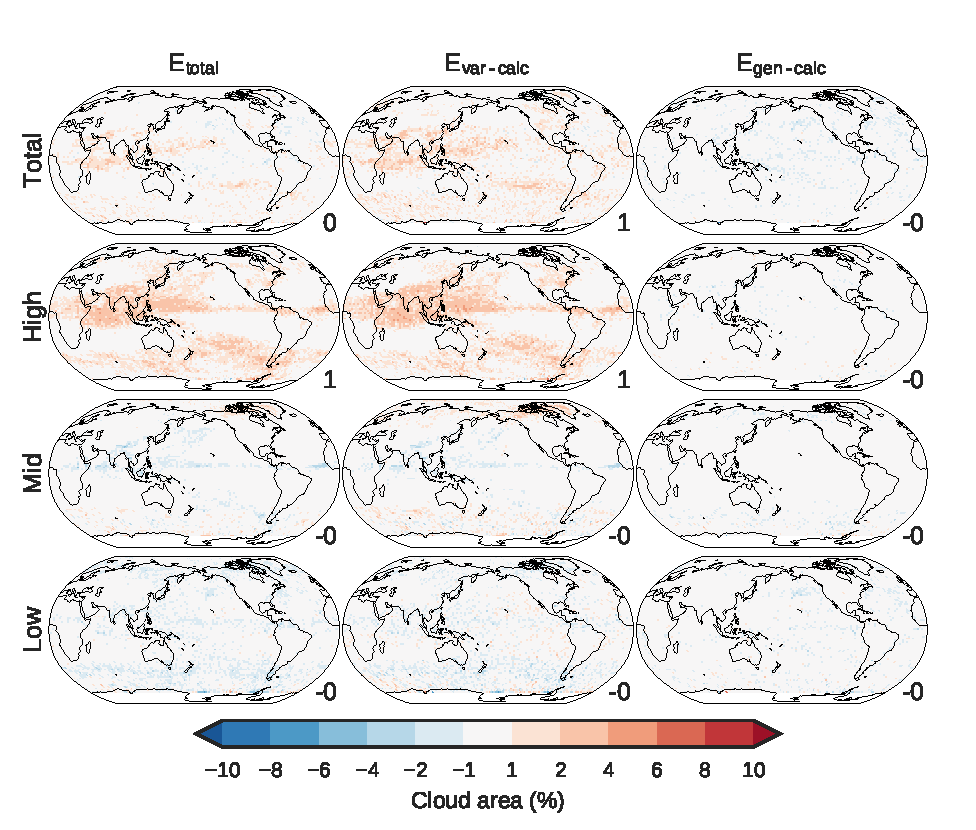
\includegraphics{graphics/subgrid2_cldmisr_maps_gen-var-calc_diff.pdf}
\caption{\label{fig:cldmisrMapsCalcDiff}Errors in MISR-simulated cloud
area by cloud top height arising due to using the improved subcolumn
generator with \emph{calculated} overlap and variability to regenerate
subcolumns from gridbox-mean profiles (left), the component of the error
due to the treatment of variability (middle), and the component of the
error due to the treatment of overlap
(right).}\label{fig:cldmisrMapsCalcDiff}
\end{figure}

\begin{figure}[htbp]
\centering
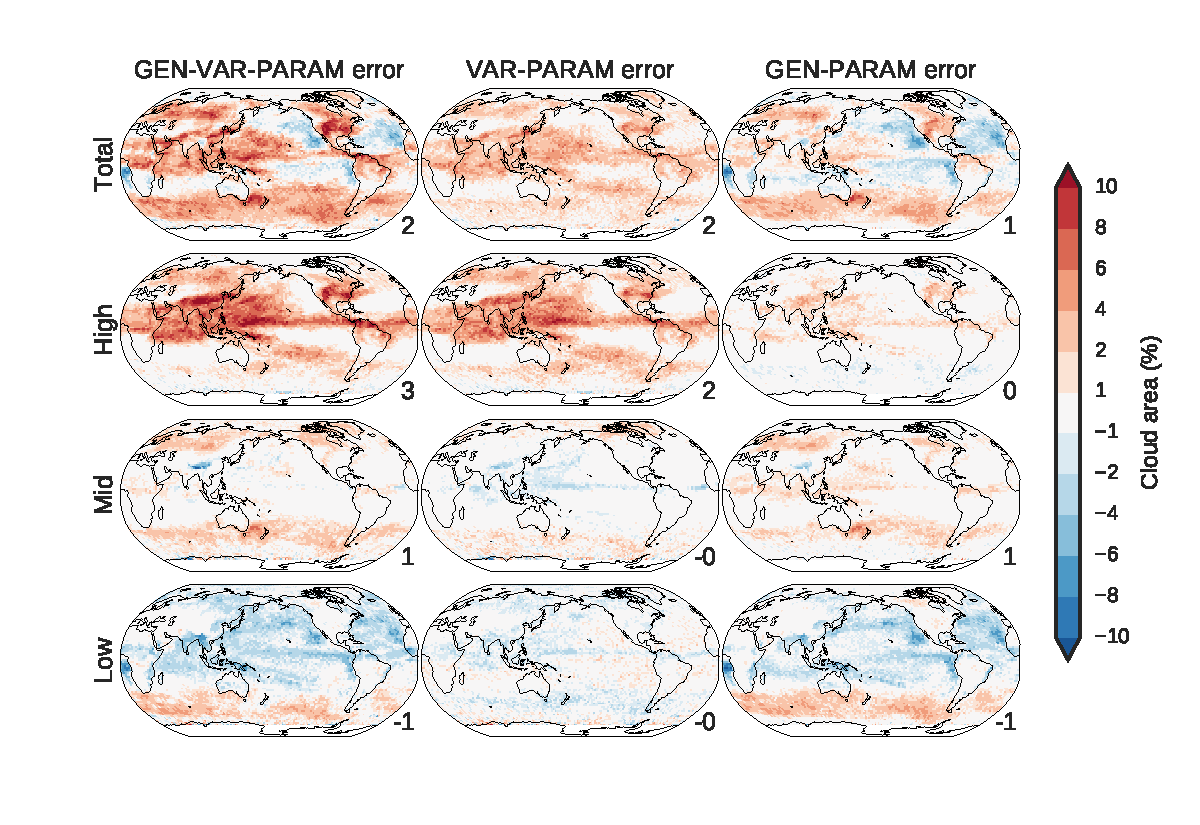
\includegraphics{graphics/subgrid2_cldmisr_maps_gen-var-param_diff.pdf}
\caption{\label{fig:cldmisrMapsParamDiff}Errors in MISR-simulated cloud
area by cloud top height arising due to using the improved subcolumn
generator with \emph{parameterized} overlap and variability to
regenerate subcolumns from gridbox-mean profiles (left), the component
of the error due to the treatment of variability (middle), and the
component of the error due to the treatment of overlap
(right).}\label{fig:cldmisrMapsParamDiff}
\end{figure}

Figure~\ref{fig:cldmisrMapsCalcDiff} and
Figure~\ref{fig:cldmisrMapsParamDiff} show the errors in MISR-simulated
cloud area by cloud top height that arise due to using the R04 subcolumn
generator to regenerate subcolumn cloud and precipitation condensate
fields from gridbox-mean profiles. Figure~\ref{fig:cldmisrMapsCalcDiff}
shows the errors in using the subcolumn generator with ideal or
``best-case'' overlap, rank correlation, and variance calculated
directly from the original CRM fields (GEN-VAR-CALC), while
Figure~\ref{fig:cldmisrMapsParamDiff} shows the errors in using the new
scheme with these quantities parameterized as discussed in
Section~\ref{sec:subgrid2Overlap} and
Section~\ref{sec:subgrid2Variability}. Comparing
Figure~\ref{fig:cldmisrMapsCalcDiff} and
Figure~\ref{fig:cldmisrMapsMroDiff} it is clear that the new scheme
(with ideal overlap and variability) is able to dramatically reduce the
errors identified in Chapter 3 in regard to total error (left-most
column), as well as due to both the treatment of variability (middle)
and overlap (right-most column). The reduction in both variability and
overlap errors means that the reduced error in the total is \emph{not}
due to a cancellation of errors (in contrast to the errors shown in
Chapter 3 that arise due to using homogeneous condensate with
maximum-random overlap). Errors due to the treatment of variability
(middle column) are everywhere less than 6\% cloud area (and generally
much smaller, between 0 and 2\%) using the new scheme, compared with
errors as large as 10\% cloud area using homogeneous condensate
(Figure~\ref{fig:cldmisrMapsMroDiff}). Errors due to the overlap
treatment are similarly reduced, from regional errors as large as 10\%
using MRO down to less than 2\% using the new scheme.

Using parameterized overlap, rank correlation, and variance results in
larger errors than using the calculated values, as seen in
Figure~\ref{fig:cldmisrMapsParamDiff}. The errors due to the treatment
of variability are comparable to those that result from using
homogeneous condensate (see Figure~\ref{fig:cldmisrMapsMroDiff}).
High-topped cloud especially is overestimated throughout the tropical
western pacific. This is likely a consequence of the parameterization of
the variance in cloud ice (and liquid, to a lesser extent) failing to
capture the large spread of condensate values present in the original
CRM fields. This is evident in the normalized CDFs shown in the right
panel of Figure~\ref{fig:mxratioCDF2}, which shows that using the
parameterization results in an underestimation of cloud ice with values
much lower than the mean.

Errors due to using parameterized overlap show clear spatial patterns,
with overestimation of cloud area especially in the southern ocean but
also somewhat in the tropical western pacific and over the continents,
and an underestimation of cloud area elsewhere. The majority of these
errors (especially in the southern ocean) appear to be in the low-topped
cloud area. These errors, especially in the southern ocean low-topped
cloud, have a similar spatial structure to the global map of
decorrelation length shown in Figure~\ref{fig:overlap_map_dz}. The
errors due to using the parameterized overlap suggest that using a
globally constant decorrelation length for cloud occurrence overlap is
insufficient to characterize the overlap of clouds simulated by SP-CAM
(and likely real clouds in the physical atmosphere).

\begin{figure}[htbp]
\centering
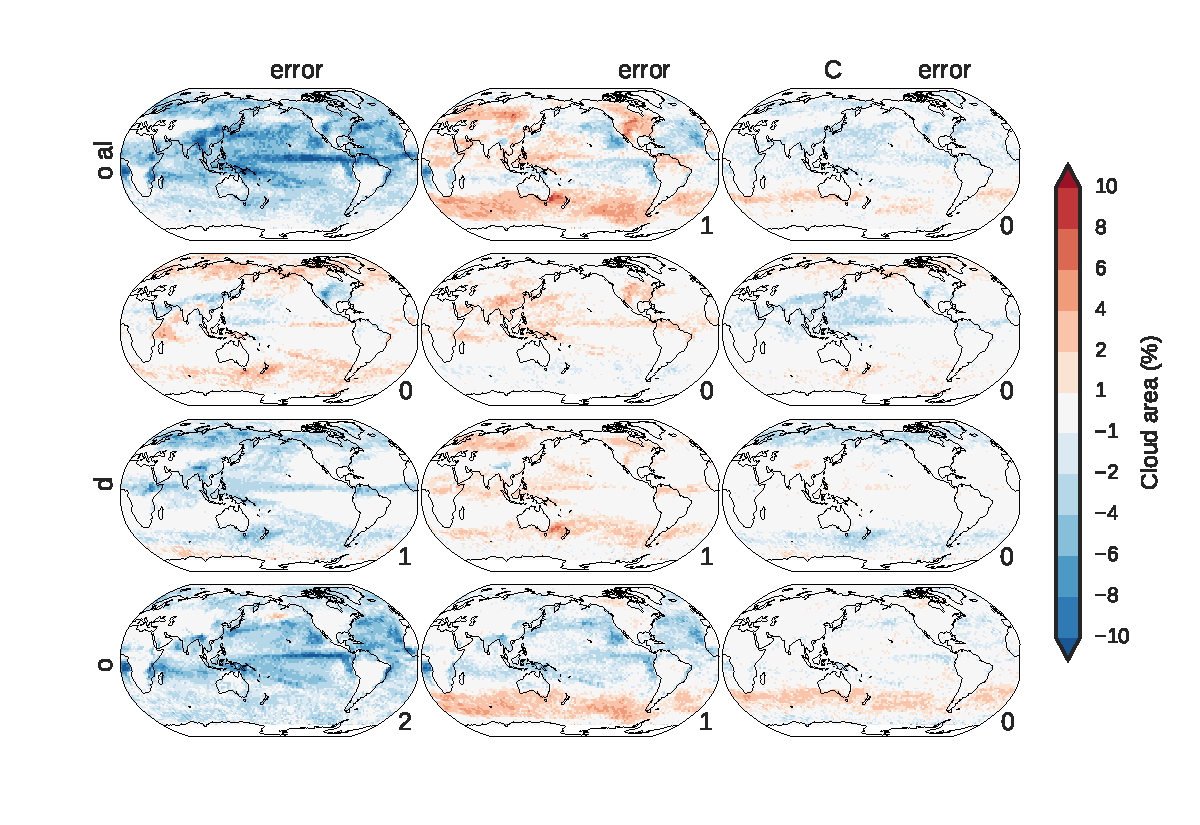
\includegraphics{graphics/subgrid2_cldmisr_maps_overlap_diff.pdf}
\caption{\label{fig:cldmisrMapsOverlapDiff}Errors in MISR-simulated
cloud area due to the parameterization of overlap alone using a constant
decorrelation length scale as described in
Section~\ref{sec:subgrid2Overlap} (\(E_\textrm{gen-param}\), far-left
column), using spatially-dependent decorrelation length scales derived
from Figure~\ref{fig:overlap_map_dz} (\(E_\textrm{gen-tab}\), middle
column), and using overlap that depends instead on temperature rather
than on separation distance, with a constant overlap (0.4) for warm
clouds and a constant overlap (0.85) for cold clouds
(\(E_\textrm{gen-const}\), far-right
column).}\label{fig:cldmisrMapsOverlapDiff}
\end{figure}

One possible alternative is to use a spatially-dependent decorrelation
scale for cloud overlap. \citep{oreopoulos_et_al_2012} use a simple
latitude-dependence to specify decorrelation lengths in their
implementation in a GCM. Taking this one step further, a
spatially-varying decorrelation length scale is tested here, using
tabulated decorrelation lengths taken from
Figure~\ref{fig:overlap_map_dz} at each latitude-longitude gridbox, and
filling in with the global average where Figure~\ref{fig:overlap_map_dz}
has missing data. The resulting errors in MISR-simulated cloud area are
shown in the middle column of Figure~\ref{fig:cldmisrMapsOverlapDiff}.
Unfortunately, these results show that even using a spatially-dependent
decorrelation length scale is insufficient, and does not result in an
appreciable reduction in errors relative to using the constant
decorrelation length.

What each of these cases lack is any dependence on cloud type, and
rather are combining the overlap effects of potentially different cloud
types or regimes together. For example, it is expected that convective
and stratiform clouds would have significantly different overlap
characteristics \citep[e.g.,][]{pincus_et_al_2005}. It would be
straightforward to implement separate overlap for convective and
stratiform clouds in GCMs that separately parameterize cloud fraction
for both of these categories, but how to do this for the SP-CAM is less
clear because the embedded CRM (SAM) does not distinguish between
convective and stratiform cloud. Instead, a simple temperature
dependence is tested here, with a single constant \emph{overlap}
\(\alpha_\textrm{cold} = 0.85\) (rather than a dependence on separation,
as studied previously) selected for levels with temperature \(t < 273\)
K, and \(\alpha_\textrm{warm} = 0.40\) for levels with temperature
\(t \ge 273\) K. The errors in MISR-simulated cloud area that result
from this simple test are shown in the far right column of
Figure~\ref{fig:cldmisrMapsOverlapDiff}. Remarkably, the errors in total
cloud area are substantially reduced using this parameterization based
on temperature, especially in the Southern Ocean. Regional errors in
cloud area are still present with this parameterization, however,
including an underestimate in high-topped cloud area throughout the
tropical western pacific (a reversal in sign from the errors in
high-topped cloud from the other two parameterizations), and a remaining
overestimation of low-topped cloud throughout the Southern Ocean. Errors
may not be eliminated with this parameterization, but the sensitivity of
the simulated MISR cloud area to changes in the parameterization of
overlap demonstrated by the different columns in
Figure~\ref{fig:cldmisrMapsOverlapDiff} suggests that these errors can
be reduced further by improving the parameterization of overlap.

While the results of Figure~\ref{fig:cldmisrMapsParamDiff} suggest that
more work needs to be done to characterize variability and overlap
statistics in order to improve MISR-simulated cloud area by cloud top
height, the results of Figure~\ref{fig:cldmisrMapsCalcDiff} demonstrate
the promise of using the improved subcolumn generator with COSP, and
suggest that future research to improve the characterization of overlap
statistics and horizontal variability in large-scale models would be a
worthwhile endeavor.

\section{Reduced errors in simulated CloudSat reflectivity and
hydrometeor occurrence}\label{sec:subgrid2Active}

\begin{figure}[htbp]
\centering
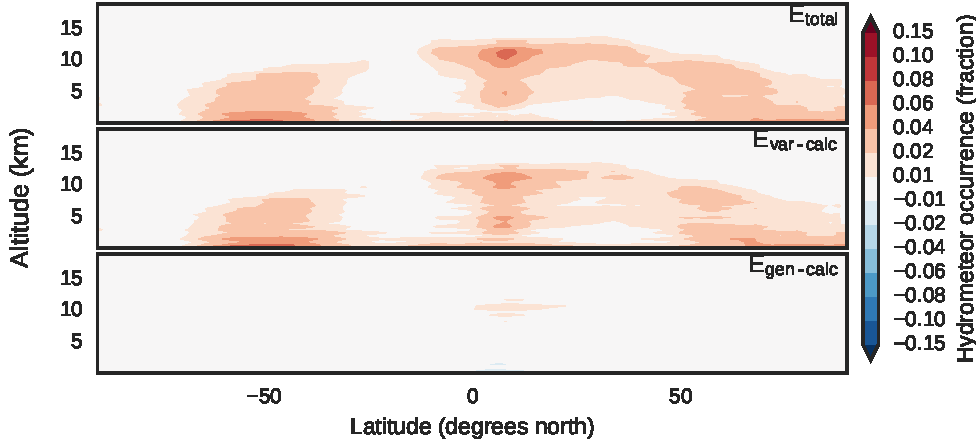
\includegraphics{graphics/subgrid2_hfba_zonal_gen-var-calc_diff.pdf}
\caption{\label{fig:hfbaZonalCalcDiff}Errors in CloudSat-simulated
hydrometeor occurrence (\(Z_e > -27.5\) dBZ) arising due to using the
improved subcolumn generator with calculated overlap and variability to
regenerate subcolumns of cloud and precipitation (top), as well as
components due to both the treatment of variability (middle) and the
treatment of overlap (bottom).}\label{fig:hfbaZonalCalcDiff}
\end{figure}

\begin{figure}[htbp]
\centering
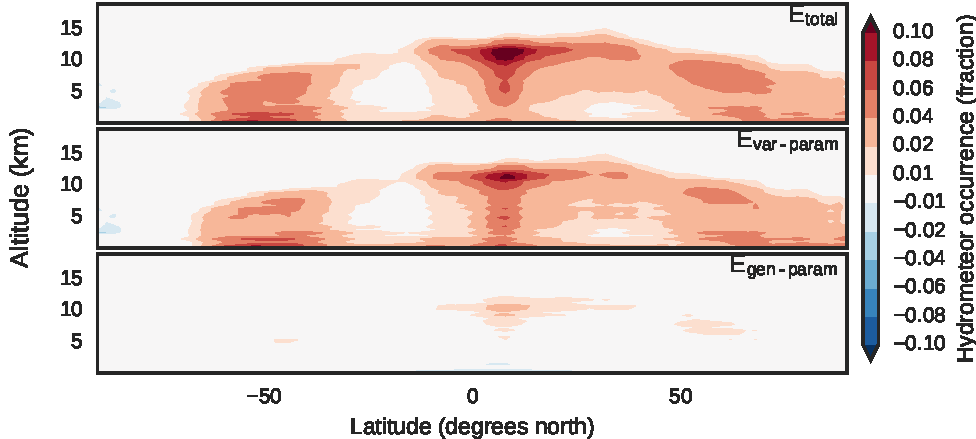
\includegraphics{graphics/subgrid2_hfba_zonal_gen-var-param_diff.pdf}
\caption{\label{fig:hfbaZonalParamDiff}Errors in CloudSat-simulated
hydrometeor occurrence (\(Z_e > -27.5\) dBZ) arising due to using the
improved subcolumn generator with parameterized overlap and variability
to regenerate subcolumns of cloud and precipitation (top), as well as
components due to both the treatment of variability (middle) and the
treatment of overlap (bottom).}\label{fig:hfbaZonalParamDiff}
\end{figure}

Figure~\ref{fig:hfbaZonalCalcDiff} and
Figure~\ref{fig:hfbaZonalParamDiff} show the errors in the
zonally-averaged CloudSat-simulated hydrometeor occurrence fraction.
Comparing these errors to those shown in
Figure~\ref{fig:hfbaZonalMroDiff} again shows a substantial reduction in
errors of all types using the improved subcolumn generator relative to
those errors that resulted from using SCOPS and PREC\_SCOPS (when using
the calculated overlap and variance). The total error that arises using
the R04 scheme with calculated overlap and variance to regenerate
subcolumns results in errors that are generally less than 0.06 frequency
of occurrence, compared to errors well above 0.1 frequency of occurrence
using the current scheme with SCOPS and PREC\_SCOPS (Chapter 3). The
remaining overestimate appears to be due to the limits of using the
gamma distribution, where (even using the exact variance) the generated
condensate amounts are too large at the low end for cloud liquid and ice
(Figure~\ref{fig:mxratioCDF2}). This inflates the area with simulated
radar reflectivity \(Z_e > -27.5\) dBZ and causes the overestimate in
hydrometeor occurrence seen in Figure~\ref{fig:hfbaZonalCalcDiff}.

Errors in CloudSat-simulated hydrometeor occurrence when using the
parameterized treatment of overlap and variability are lower than when
using the current COSP scheme (SCOPS and PREC\_SCOPS), but are
nonetheless much larger than when using the calculated overlap and
variability. This suggests that considerable improvement can be realized
with further efforts to parameterize variability. The errors due to the
treatment of overlap remain small when using the parameterization, as
one might expect given that the ``cloud masking'' effect discussed in
the previous section for simulated MISR cloud area does not apply to
CloudSat-simulated hydrometeor occurrence beyond than the effects of
attenuation (which are likely a second order effect on hydrometeor
occurrence shown here). Thus, overlap errors shown in
Figure~\ref{fig:hfbaZonalCalcDiff} and
Figure~\ref{fig:hfbaZonalParamDiff} (bottom panels) are so low that they
are barely visible on the color scale used.

\begin{figure}[htbp]
\centering
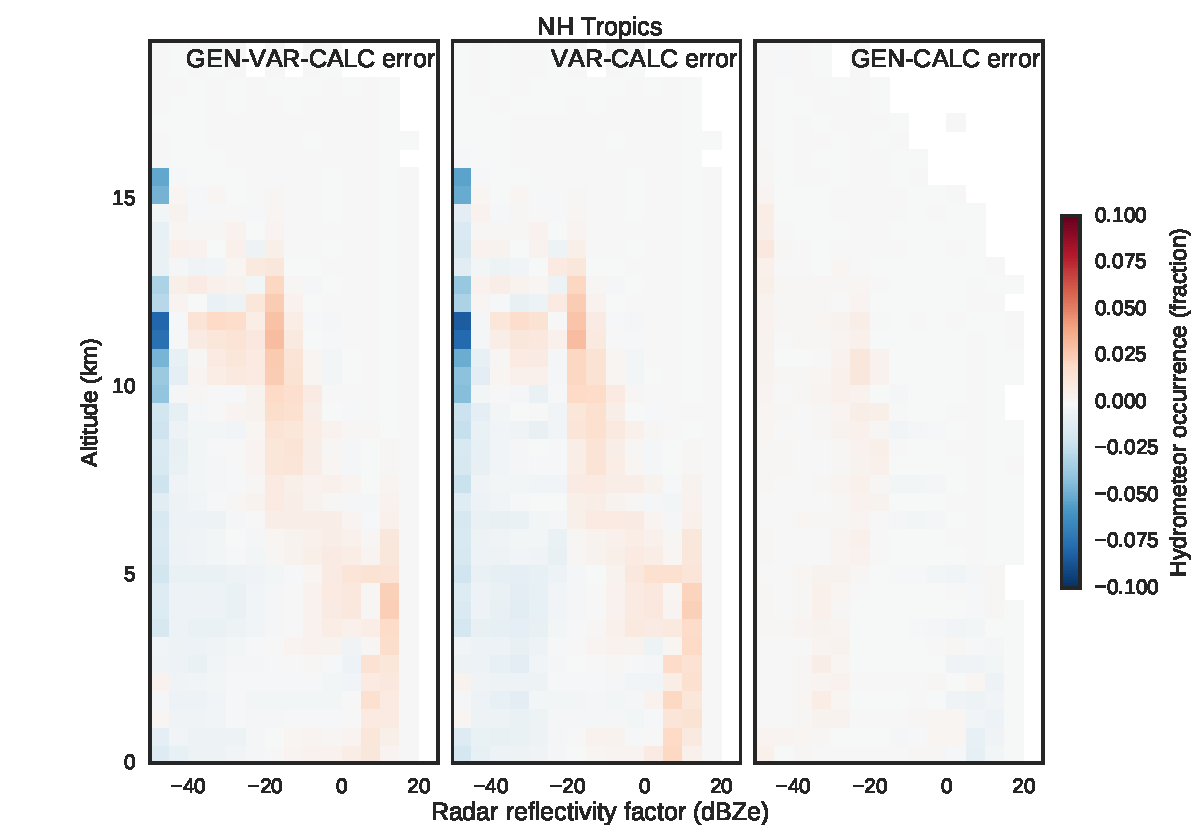
\includegraphics{graphics/subgrid2_cfadDbze94_NHTropics_gen-var-calc_diff.pdf}
\caption{\label{fig:cfadTropicsCalcDiff}Errors in CloudSat-simulated
reflectivity with height histograms for the NH Tropics (0 to 10 degrees
north).}\label{fig:cfadTropicsCalcDiff}
\end{figure}

\begin{figure}[htbp]
\centering
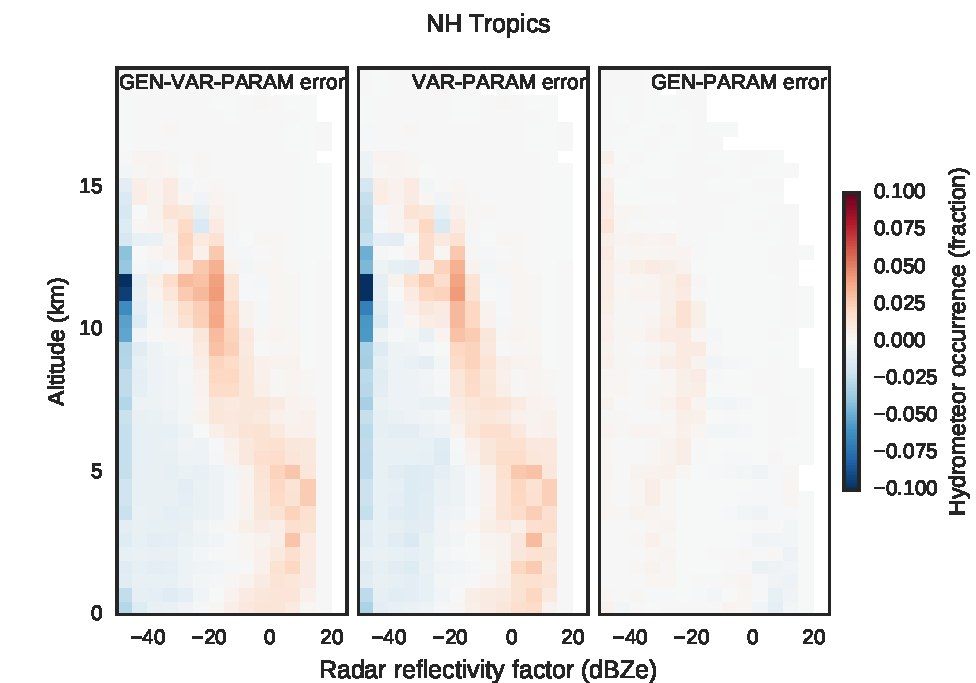
\includegraphics{graphics/subgrid2_cfadDbze94_NHTropics_gen-var-param_diff.pdf}
\caption{\label{fig:cfadTropicsParamDiff}Errors in CloudSat-simulated
reflectivity with height histograms for the NH Tropics (0 to 10 degrees
north).}\label{fig:cfadTropicsParamDiff}
\end{figure}

Figure~\ref{fig:cfadTropicsCalcDiff} and
Figure~\ref{fig:cfadTropicsParamDiff} show errors in CloudSat-simulated
reflectivity with height histograms for the northern hemisphere tropics
(0 to 10 degrees north). The figures show a reduction in errors of all
types (total error as well as components due to variability and overlap)
using the new subcolumn scheme with either calculated or parameterized
overlap and variability to regenerate subcolumns compared with the
errors identified in Figure~\ref{fig:cfadTropicsMroDiff}. Again, errors
are somewhat larger using the parameterized variance treatment, while
the error due to using the parameterized overlap treatment remains
small. These errors are somewhat different in nature than identified in
Chapter 3. While using homogeneous condensate primarily resulted in
increased frequency of occurrence along the characteristic curve in
reflectivity-height space, the errors shown in
Figure~\ref{fig:cfadTropicsParamDiff} are not entirely on the
characteristic curve. In particular, the errors at high-altitudes (where
ice is present) are primarily at smaller reflectivities, consistent with
the issues identified above with representing the full distribution of
cloud ice.

\begin{figure}[htbp]
\centering
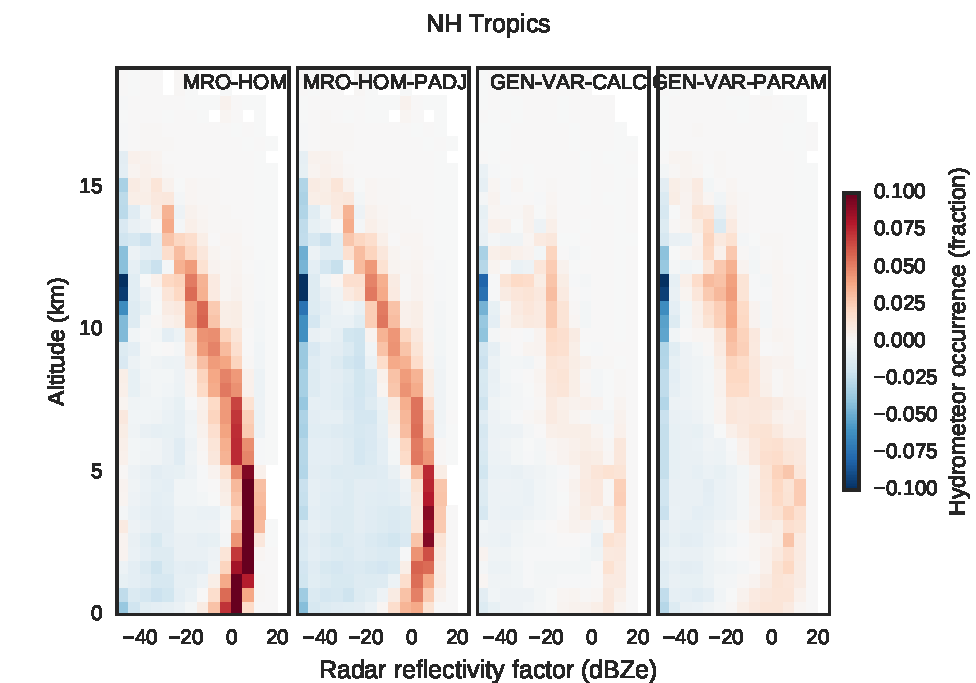
\includegraphics{graphics/subgrid2_cfadDbze94_NHTropics_all_diff.pdf}
\caption{\label{fig:cfadTropicsAllDiff}Errors in CloudSat-simulated
reflectivity with height histograms for the NH Tropics (0 to 10 degrees
north) that result from using each of four configurations of the
subcolumn generator, including, from left to right: the COSP
implementation of SCOPS and PREC\_SCOPS with homogeneous condensate and
maximum-random overlap (MRO-HOM), SCOPS and PREC\_SCOPS with adjusted
precipitation fraction (MRO-HOM-PADJ), the improved subcolumn generator
with calculated overlap and variance (GEN-VAR-CALC), and the improved
subcolumn generator with parameterized overlap and variance
(GEN-VAR-PARAM).}\label{fig:cfadTropicsAllDiff}
\end{figure}

\begin{figure}[htbp]
\centering
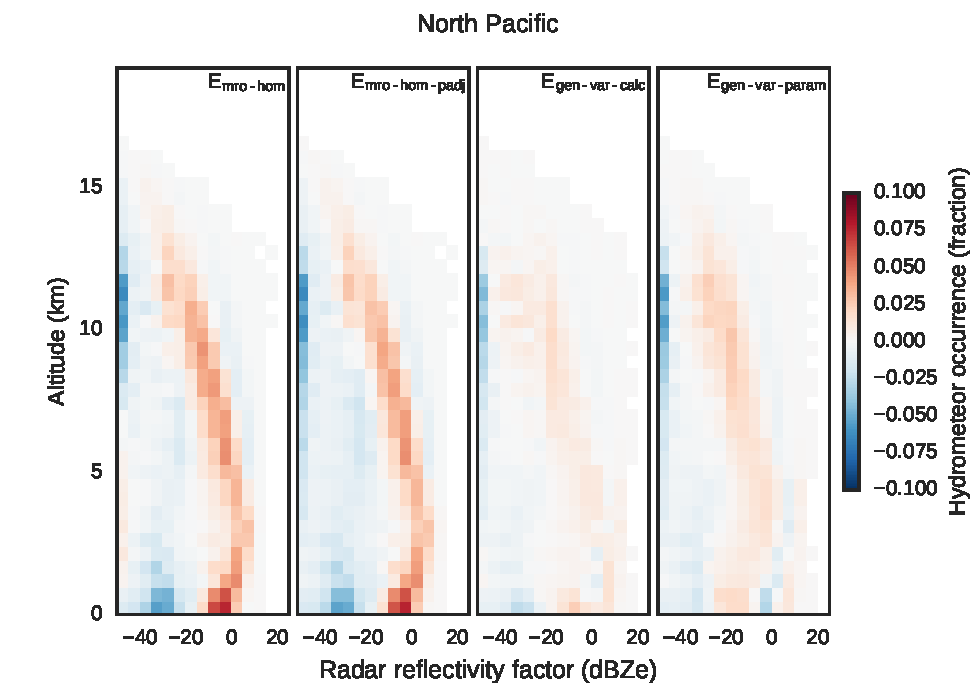
\includegraphics{graphics/subgrid2_cfadDbze94_NorthPacific_all_diff.pdf}
\caption{\label{fig:cfadNPAllDiff}Errors in CloudSat-simulated
reflectivity with height histograms for the North Pacific (35 to 60
degrees north latitude, 160 to 220 degrees east longitude) that result
from using each of four configurations of the subcolumn generator,
including, from left to right: the COSP implementation of SCOPS and
PREC\_SCOPS with homogeneous condensate and maximum-random overlap
(MRO-HOM), SCOPS and PREC\_SCOPS with adjusted precipitation fraction
(MRO-HOM-PADJ), the improved subcolumn generator with calculated overlap
and variance (GEN-VAR-CALC), and the improved subcolumn generator with
parameterized overlap and variance
(GEN-VAR-PARAM).}\label{fig:cfadNPAllDiff}
\end{figure}

The errors shown in Figure~\ref{fig:hfbaZonalParamDiff} and
Figure~\ref{fig:cfadTropicsParamDiff} that arise from using the simple
parameterization of condensate variability presented here show that
improvements to this parameterization are needed to accurately
characterize the condensate heterogeniety, but these errors are still
substantially smaller than arise when using homogeneous condensate,
especially for the full reflectivity with height histograms.
Figure~\ref{fig:cfadTropicsAllDiff} shows the total errors for the NH
Tropics from using each configuration of subcolumn generators, including
SCOPS and PREC\_SCOPS (MRO-HOM, far-left column), SCOPS and PREC\_SCOPS
with the precipitation adjustment (MRO-HOM-PADJ, second column), the new
subcolumn generator with calculated overlap and variance (GEN-VAR-CALC,
third column), and the new subcolumn generator with parameterized
overlap and variance (GEN-VAR-PARAM, far-right column).
Figure~\ref{fig:cfadNPAllDiff} shows the same cases but for the North
Pacific region. It is obvious that although the errors using
parameterized overlap and variance are larger than when using calculated
overlap and variance, these errors are much smaller than when using
SCOPS and PREC\_SCOPS with homogeneous condensate, especially at
lower-altitudes.

\section{Discussion}\label{sec:subgrid2Discussion}

In this chapter, a new cloud subcolumn generator using the algorithm of
\citet{raisanen_et_al_2004} has been presented to potentially replace
the current implementation of SCOPS in COSP. The new subcolumn generator
allows for a more realistic representation of cloud overlap by
representing overlap as a linear combination of maximum and random
overlap, as well as horizontally variable cloud and precipitation
condensate amount sampled from gamma distributions. The impact of these
changes on simulated satellite-observable cloud diagnostics from COSP
has been evaluated by using the new subcolumn generator to regenerate
subcolumns of cloud and precipitation condensate from CRM output from
SP-CAM that has been averaged to mimic gridbox mean quantities as would
be represented by a traditional GCM. These impacts have been tested both
with idealized overlap and horizontal variability calculated directly
from the original CRM fields and with overlap and horizontal variability
parameterized.

The sensitivity test framework uses outputs from the SP-CAM to provide a
plausible representation of cloud and precipitation structure and
variability at scales similar to those at which the satellite retrievals
are performed. While these outputs provide much higher resolution cloud
fields than available in traditional GCMs, the fields simulated by the
SP-CAM are in fact still model outputs, and may not perfectly simulate
any observed cloud systems. Nonetheless, the overlap and condensate rank
correlation statistics from SP-CAM are consistent with those found in
observations from previous authors, and condensate variability is
consistent with previous studies as well, following similar statistical
distributions. Thus, since the goal of this study is to evaluate the
sensitivity of COSP diagnostics to these properties, rather than to
develop a perfect parameterization of subgrid-scale overlap and
variability, the SP-CAM output is sufficient for this purpose. In order
to run the individual simulators directly on output from the SP-CAM, it
is important that the fields simulated by the SP-CAM are on a scale
similar to that at which the satellite retrievals are performed. The
SP-CAM output used in this study was run using 4 km grid spacing for the
embedded cloud-resolving model. MISR cloud top height retrievals are
performed at a spatial scale of 1.1 km \citep{moroney_et_al_2002}, and
the CloudSat cloud radar has a horizontal resolution of 1.4 km
cross-track and 1.7 km along-track \citep{tanelli_et_al_2008}. While
these scales are somewhat smaller than the 4 km grid used by the SP-CAM
CRM, the differences are small and are unlikely to affect the results of
the sensitivity study performed with the 4 km fields.

The ceiling of potential performance of the new subcolumn scheme is
demonstrated by running COSP on subcolumns regenerated with overlap and
variability calculated directly from the original CRM fields. It has
been shown here that this leads to substantial improvements in
satellite-simulated cloud properties. This suggests that implementing
this framework can substantially reduce errors in simulated clouds that
arise due to the currently used assumptions of maximum-random overlap
and horizontally homogeneous cloud and precipitation (as shown in the
previous chapter).

It is clear that the parameterization leaves a lot of room for
improvement, but it is stressed that the purpose here is not to develop
a perfect parameterization that can be immediately implemented into a
large-scale model, but rather to demonstrate the sensitivity of
satellite-simulated diagnostics from COSP to improvements in the
treatment of variability and overlap. The simple parameterization
presented here is sufficient to accomplish this.

While results using the ideal (calculated) overlap and variability from
the original CRM fields demonstrate the potential of the new subcolumn
generator, results using the parameterized overlap and variability show
that the performance of the subcolumn generator is somewhat dependent on
how overlap and variability are parameterized within this framework. In
particular, it appears that MISR-simulated cloud area by cloud top
height is dependent on both the representation of variability and of
overlap, while CloudSat-simulated radar reflectivity is primarily
dependent on the representation of variability (and precipitation
occurrence, as demonstrated in the previous chapter). Large errors arise
when parameterizing overlap and rank correlation as functions of
separation distance alone with constant decorrelation length scales, and
assuming constant decorrelation length scales is insufficient for
capturing the overlap characteristics of clouds simulated by SP-CAM (see
Figure~\ref{fig:overlap_map_dz} and Figure~\ref{fig:rankcorr_maps_dz}).
However, substantially better results are demonstrated when using
overlap that depends instead on temperature, with separate (still
spatially-invariant) values of the overlap parameter \(\alpha\) for warm
and cold clouds, suggesting that further improvements can be made by
parameterizing overlap as a function of not just separation but on
additional aspects of the gridbox as well. Many questions about how best
to represent overlap statistics remain, and this will be an interesting
area of future research.

Errors arising due to the parameterization of variability presented here
remain significant for both MISR-simulated cloud area by cloud top
height and for CloudSat-simulated hydrometeor occurrence, demonstrating
the need for continued efforts to improve parameterization of overlap
and variability. Errors in CloudSat-simulated reflectivity with height
are notably reduced even with the crude parameterization of variability
presented here.

These issues are not unique to simulation of satellite-observable cloud
diagnostics, and it has been recognized that subgrid-scale variability,
including cloud and precipitation occurrence overlap and condensate
amount, effect many important processes in large-scale models, and some
researchers are trying to develop explicit subgrid treatments for GCMs.
This includes so-called ``statistical'' or ``assumed probability
distribution'' schemes, which predict the evolution of not only the
mean, but also the probability distribution of total water (and to a
degree the cloud and precipitation condensate) within each grid-box
\citep[e.g.,][]{tompkins_2002}. There has been growing interest in using
these schemes in GCMs. One such example of this is the Cloud Layers
Unified By Binormals \citep[CLUBB;][]{golaz_et_al_2002} scheme, which is
being implemented into the NCAR CAM (A. Gettelman, personal
communication). Because these schemes are formulated using a probability
distribution for the subgrid variability of condensate, they are a
natural fit to the stochastic treatment of subgrid clouds and
precipitation used in COSP to simulate satellite retrievals (and also to
radiation schemes that use stochastic treatments of subgrid clouds such
as the McICA \citep{pincus_et_al_2003}, because the same distribution of
condensate can be shared between these different components of the
model. As shown here for simulated satellite diagnostics and by others
for calculated radiative fluxes, these assumptions can have a large
impact on diagnosed cloud effects, and thus consistency between cloud
treatments in the different parts of the model is necessary in order to
obtain a consistent picture of the performance of models in simulating
clouds.
